%% bare_conf.tex
%% V1.3
%% 2007/01/11
%% by Michael Shell
%% See:
%% http://www.michaelshell.org/
%% for current contact information.
%%
%% This is a skeleton file demonstrating the use of IEEEtran.cls
%% (requires IEEEtran.cls version 1.7 or later) with an IEEE conference paper.
%%
%% Support sites:
%% http://www.michaelshell.org/tex/ieeetran/
%% http://www.ctan.org/tex-archive/macros/latex/contrib/IEEEtran/
%% and
%% http://www.ieee.org/

%%*************************************************************************
%% Legal Notice:
%% This code is offered as-is without any warranty either expressed or
%% implied; without even the implied warranty of MERCHANTABILITY or
%% FITNESS FOR A PARTICULAR PURPOSE!
%% User assumes all risk.
%% In no event shall IEEE or any contributor to this code be liable for
%% any damages or losses, including, but not limited to, incidental,
%% consequential, or any other damages, resulting from the use or misuse
%% of any information contained here.
%%
%% All comments are the opinions of their respective authors and are not
%% necessarily endorsed by the IEEE.
%%
%% This work is distributed under the LaTeX Project Public License (LPPL)
%% ( http://www.latex-project.org/ ) version 1.3, and may be freely used,
%% distributed and modified. A copy of the LPPL, version 1.3, is included
%% in the base LaTeX documentation of all distributions of LaTeX released
%% 2003/12/01 or later.
%% Retain all contribution notices and credits.
%% ** Modified files should be clearly indicated as such, including  **
%% ** renaming them and changing author support contact information. **
%%
%% File list of work: IEEEtran.cls, IEEEtran_HOWTO.pdf, bare_adv.tex,
%%                    bare_conf.tex, bare_jrnl.tex, bare_kernel_comp soc.TeX
%%*************************************************************************

% *** Authors should verify (and, if needed, correct) their LaTeX system  ***
% *** with the test flow diagnostic prior to trusting their LaTeX platform ***
% *** with production work. IEEE's font choices can trigger bugs that do  ***
% *** not appear when using other class files.                            ***
% The test flow support page is at:
% http://www.michaelshell.org/tex/testflow/

% Note that the a4paper option is mainly intended so that authors in
% countries using A4 can easily print to A4 and see how their papers will
% look in print - the typesetting of the document will not typically be
% affected with changes in paper size (but the bottom and side margins will).
% Use the test flow package mentioned above to verify correct handling of
% both paper sizes by the user's LaTeX system.
%
% Also note that the "draft cls" or "draftclsnofoot", not "draft", option
% should be used if it is desired that the figures are to be displayed in
% draft mode.

\documentclass[10pt, conference, compsocconf]{IEEEtran}
\usepackage{xltxtra}
\usepackage{subfig}
\usepackage{booktabs}
\usepackage{amsmath}
\usepackage{flushend}
\usepackage[numbers,sort&compress]{natbib}
\setmainfont{Times New Roman}

\begin{document}

\title{igrow: A Multithreaded Ligand Growing Tool for Structure-Based Molecule Design} % can use linebreaks \\ within to get better formatting as desired
\author
{
\IEEEauthorblockN
{
Hongjian Li\IEEEauthorrefmark{1}, Ching-Man Tse\IEEEauthorrefmark{1}, Kwong-Sak Leung\IEEEauthorrefmark{1}, Man-Hon Wong\IEEEauthorrefmark{1}, Kin-Hong Lee\IEEEauthorrefmark{1} and Mary Miu-Yee Waye\IEEEauthorrefmark{2}
\IEEEauthorblockA
{
\IEEEauthorrefmark{1}
Department of Computer Science and Engineering, Chinese University of Hong Kong, Hong Kong, P.R. China\\
\{hiji, cmtse, ksleung, mhwong, khlee\}@cse.cuhk.edu.hk
}
\IEEEauthorblockA
{
\IEEEauthorrefmark{2}
School of Biomedical Sciences, Chinese University of Hong Kong, Hong Kong, P.R. China\\
mary-waye@cuhk.edu.hk
}
}
}
\maketitle

\begin{abstract}



\end{abstract}

\begin{IEEEkeywords}

bioinformatics, chemoinformatics, drug discovery, molecular docking, virtual screening, multithreading

\end{IEEEkeywords}

\section{Introduction}

As the X-ray crystallography technology evolves, more and more structures of biological macromolecules at atomic level have been revealed and deposited into the world's largest repository Protein Data Bank (PDB) \cite{539,537}. This rapid evolution catalyzes the development of various protein-ligand docking tools for structure-based drug discovery.

Protein-ligand docking is a method which predicts the preferred conformation of a small ligand when bound to a macro protein to form a stable complex. It also predicts the binding affinity in terms of free energy, which is basically the overall effect of various chemical forces involved. The lower the free energy, the higher the binding affinity. Very often, the target protein is a viral enzyme of interest, and the small organic ligands that are predicted to inhibit the viral enzyme are what we want to discover. Structure-based virtual screening is simply a massive version of docking. It docks a database of drug-like ligands to a target, ranks them according to their predicted binding affinity, and shortlists the best ones for further investigation.

\section{Motivation}



\section{Problem Definition}



\section{Method}

Figure \ref{fig:Flowchart} shows the overall flowchart of igrow. 

\begin{figure}
\centering
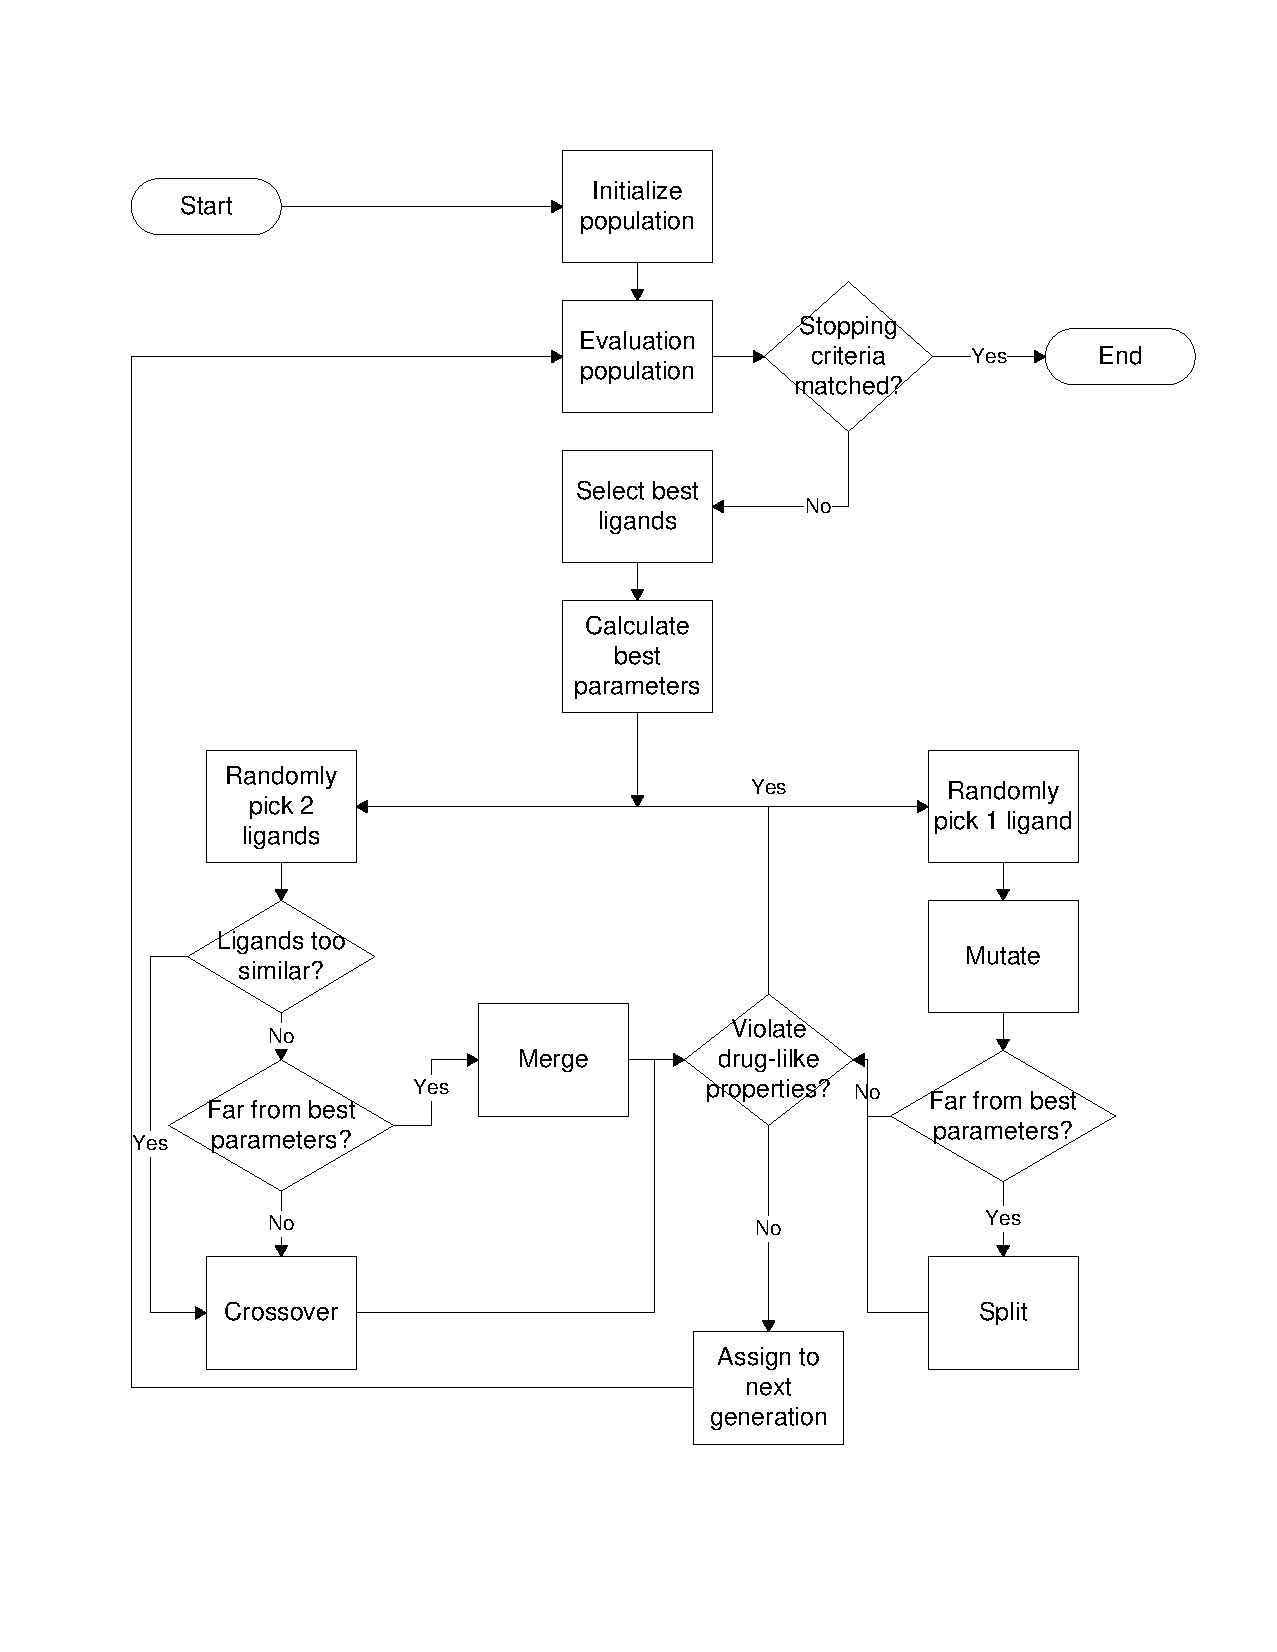
\includegraphics[width=\linewidth]{Figures/Methods/Flowchart.pdf}
\caption{Flowchart of igrow.}
\label{fig:Flowchart}
\end{figure}

\subsection{Genetic Operators}



\subsection{idock}

Grid map reuse.

Both idock and Vina use Monte Carlo algorithm for global optimization and Broyden-Fletcher-Goldfarb-Shanno (BFGS) \cite{786} Quasi-Newton method for local optimization. Both programs achieve multithreading by concurrently running multiple independent Monte Carlo tasks starting from random initial conformations.

\subsection{C++ Implementation Tricks}

igrow remarkably revises the fundamental C++ implementation. idock invents its own thread pool in order to reuse threads and maintain a high CPU utilization throughout the entire screening procedure. The thread pool parallelizes the creation of grid maps and the execution of Monte Carlo tasks. idock estimates the capacity of every vector structure and intensively utilizes Rvalue reference, a new feature in the C++11 standard, to avoid frequent memory reallocation. idock flattens Vina's tree-like recursive data structure of ligand into simple linear array structure to ensure a high data cache hit rate and easy coding. idock accelerates the assignment of atom types by making use of residue information for receptor and branch information for ligand, without explicitly detecting covalent bonds among atoms.

\section{Data}

In order to test igrow comprehensively, we collected 3 receptors from PDB \cite{96} and 8 unique initial ligands from PDB and ZINC \cite{55}. From these data, 18 test cases could be formed, as detailed below.

\subsection{Receptors}

We aim to select receptors that are of real-life importance. Glycogen synthase kinase 3 beta (GSK3$\beta$) is a theoretically promising pharmacotherapeutic target for the treatment of several human diseases, including type-2 diabetes \cite{247} and Alzheimer's disease (AD) \cite{248}. Efforts into discovering new inhibitors of GSK3$\beta$ never stop \cite{246}. Therefore it was included into our test data.

HIV was also selected for its impact to human kind. According to the latest fact sheets of World Health Organization in 2010, 33.4 million people live with HIV/AIDS worldwide. HIV reverse transcriptase (HIV RT) and HIV protease (HIV PR), two viral proteins residing in the body of the virus, assist the virus in infecting human cells. Researchers have spent over 30 years in discovering new inhibitors of HIV RT and HIV PR \cite{221,222,223}. Therefore, they were also included into our test data.

Totally 3 receptors were collected from PDB \cite{96} for testing. They are glycogen synthase kinase 3 beta (GSK3$\beta$) of PDB ID 1J1B \cite{245} of resolution 1.80 \AA, HIV reverse transcriptase (HIV RT) of PDB ID 2ZD1 \cite{180} of resolution 1.80 \AA, and HIV protease (HIV PR) of PDB ID 3KFN \cite{243} of resolution 1.77 \AA.

We manually extracted the 3 receptors out of their PDB complexes, and queried CSA (Catalytic Site Altas) \cite{206} and relevant publications \cite{245,246,180,221,222,223,243} for their possible binding sites, as shown in table \ref{tab:searchspace}.

\begin{table*}
\centering
\begin{tabular*}
{\linewidth}
{@{\extracolsep{\fill}}lccc}
\noalign{\smallskip}
\toprule
Receptor & Glycogen synthase kinase 3 beta & HIV reverse transcriptase & HIV protease\\
\midrule
\noalign{\smallskip}
PDB ID & 1J1B & 2ZD1 & 3KFN\\
Resolution & 1.80 \AA & 1.80 \AA & 1.77 \AA\\
Selected binding site & Catalytic site & Allosteric site for NNRTI binding & Exo site\\
Grid box center & (20.304 \AA, 16.365 \AA, -9.814 \AA) & (49.712 \AA, -28.441 \AA, 35.555 \AA) & (8.113 \AA, 9.701 \AA, 4.310 \AA) \\
Grid box size & 22 x 18 x 20 \AA$^3$ & 16 x 16 x 18 \AA$^3$ & 22 x 26 x 22 \AA$^3$\\
\bottomrule
\end{tabular*}
\caption{PDB IDs, resolutions, selected binding sites, grid box centers and sizes of the 3 testing receptors. NNRTI stands for non-nucleotide reverse transcriptase inhibitor. The exo site of HIV protease refers to the exo site adjacent to the Gly$^{16}$Gly$^{17}$Gln$^{18}$ loop.}
\label{tab:searchspace}
\end{table*}

\subsection{Initial Ligands}

We aimed to select initial ligands that spread across wide ranges of free energies and molecular weights. The 3 ligands of PDB heterogeneous molecule IDs TRS, T27 and 4DX are respectively native ligands of GSK3$\beta$, HIV RT and HIV PR, hence they were included.

Additionally, we retrieved 5 more ligands from ZINC \cite{55}, namely ZINC01019824, ZINC08442219, ZINC09365179, ZINC18153302, and ZINC20030231. The free energies and molecular weights of these 5 ligands spread across a wide range.

Totally 8 unique initial ligands were chosen, as shown in figure \ref{fig:UniqueInitialLigands}. The 5 ZINC ligands were repeatedly used as initial ligands for each of the 3 receptors, resulting in a total of 18 initial ligands under the context of the 3 receptors. Note that even for the same ZINC initial ligand, its predicted free energy varies when docking to different receptors.

\begin{figure*}
\centering
\subfloat[TRS]
{
  \label{subfig:Ligands-TRS}
  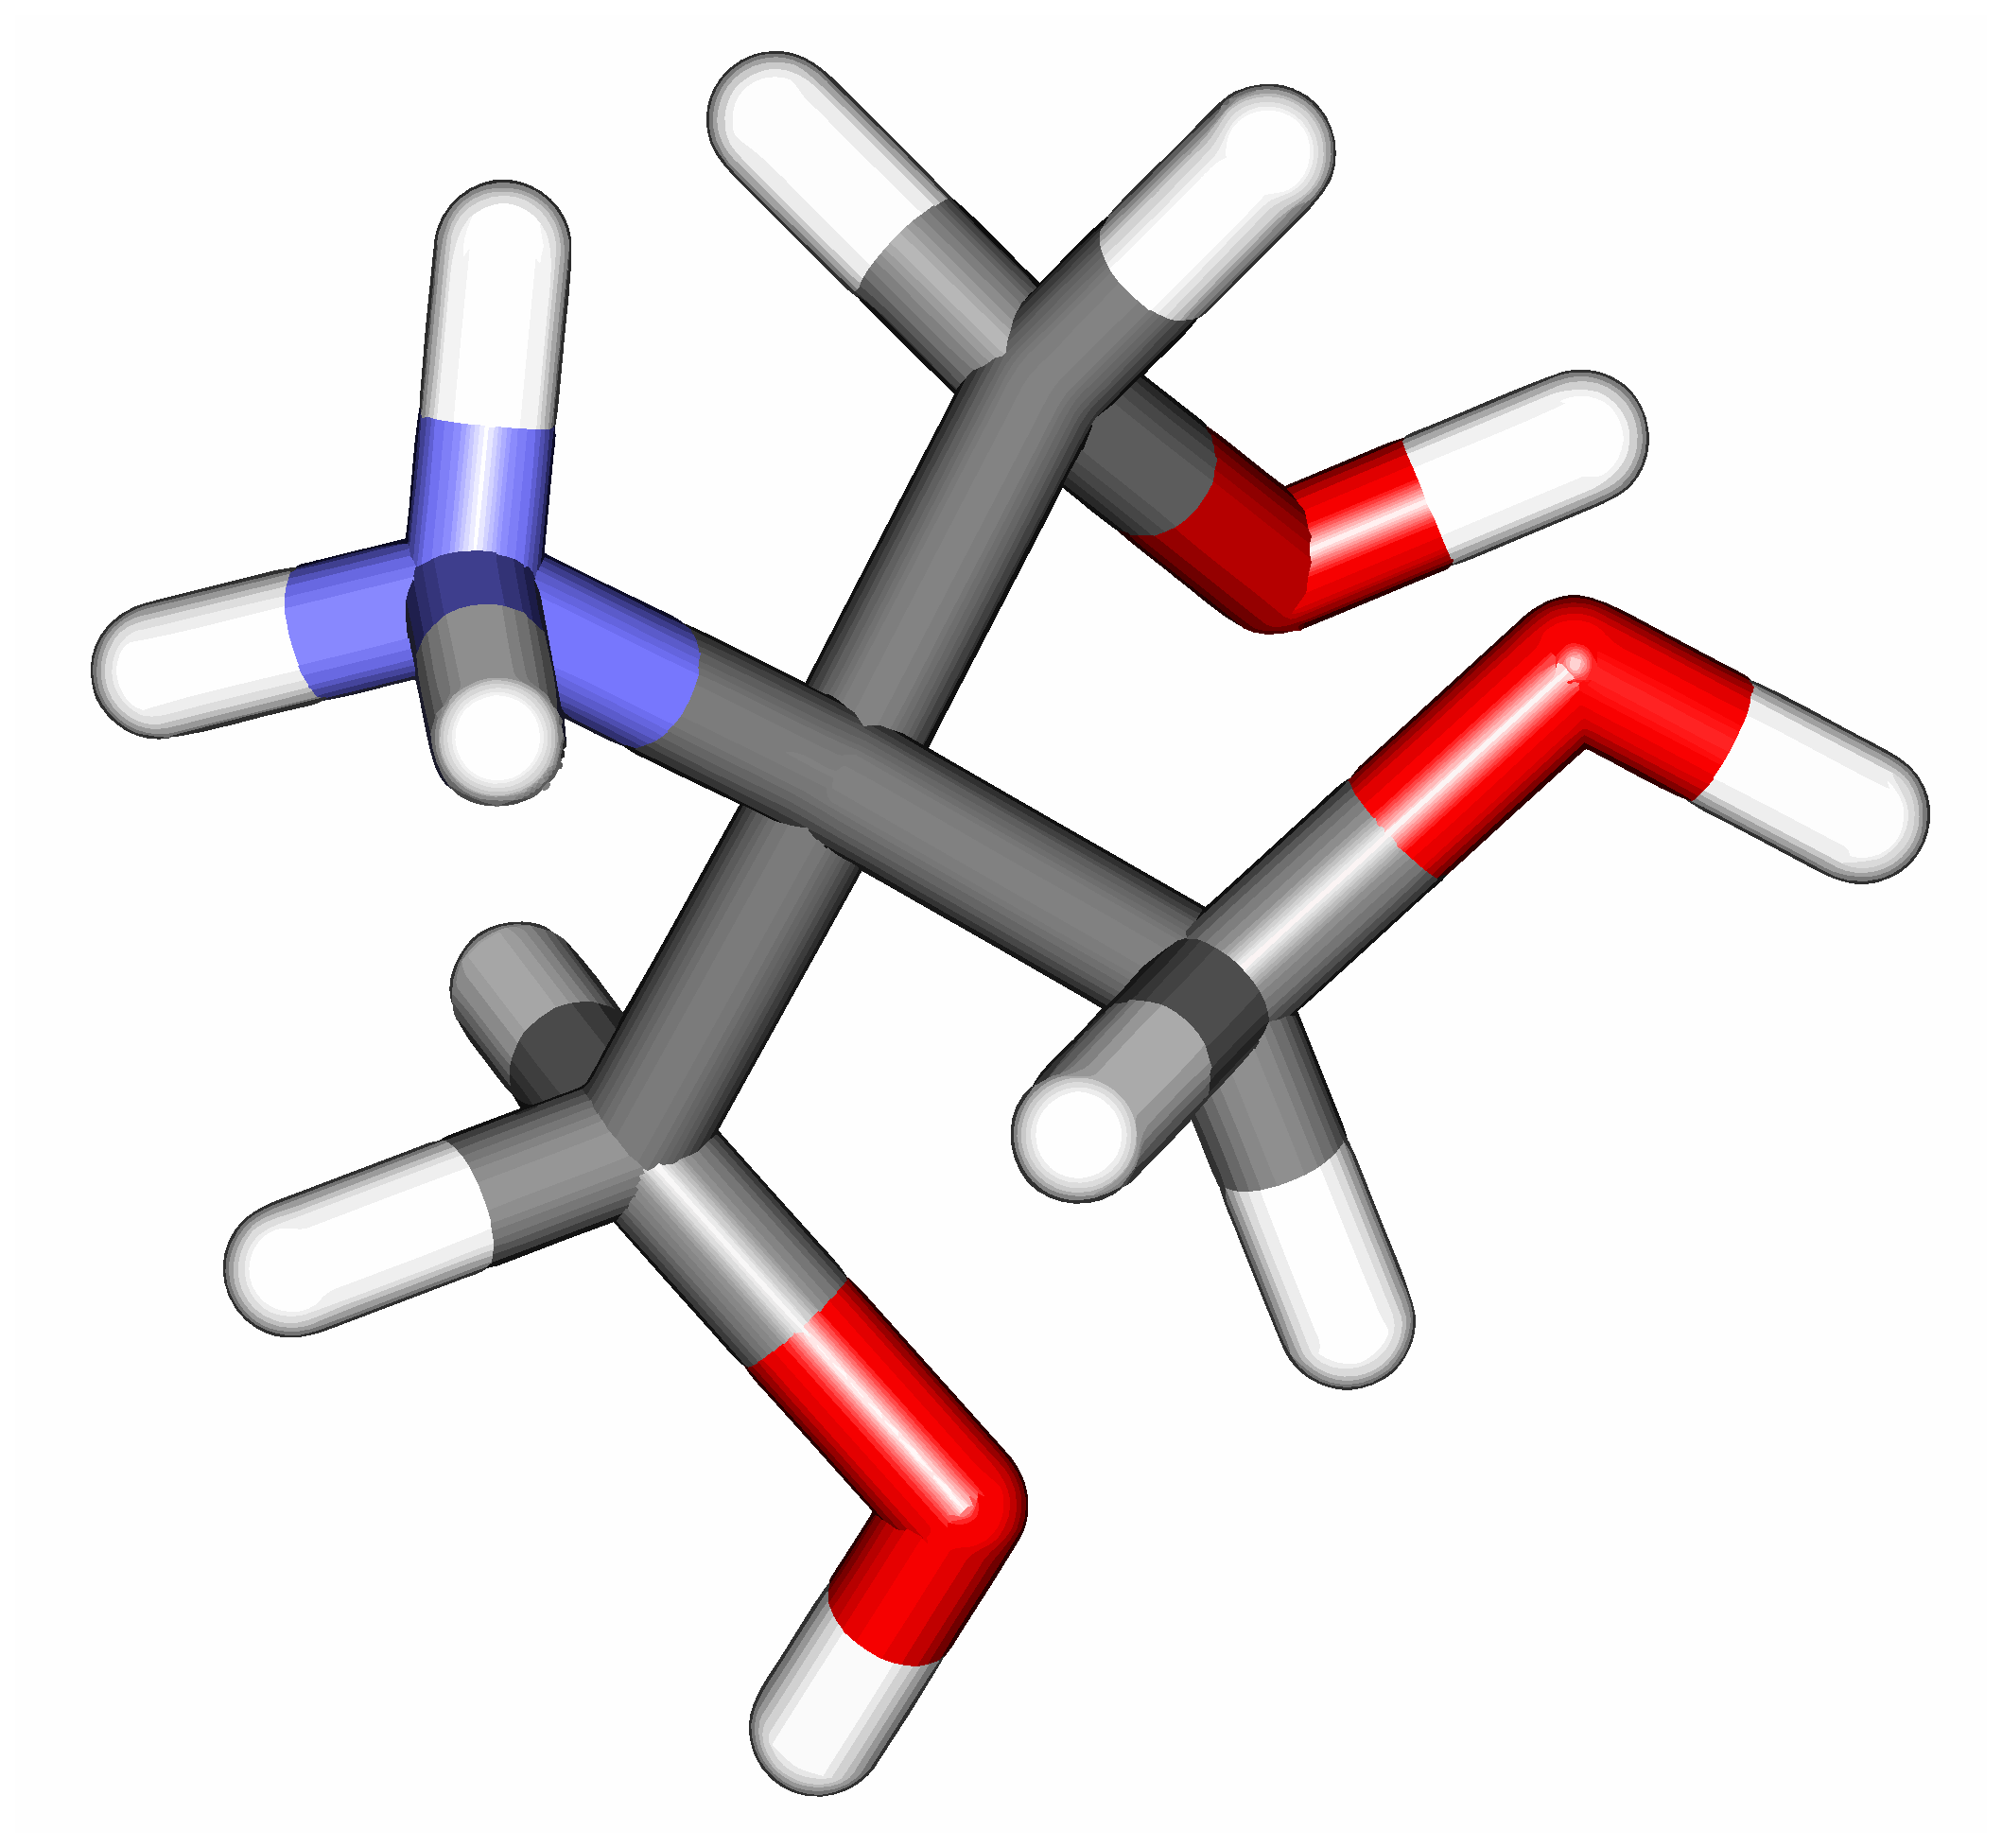
\includegraphics[width=0.11\linewidth]{Figures/Ligands/TRS.eps}
}
\subfloat[T27]
{
  \label{subfig:Ligands-T27}
  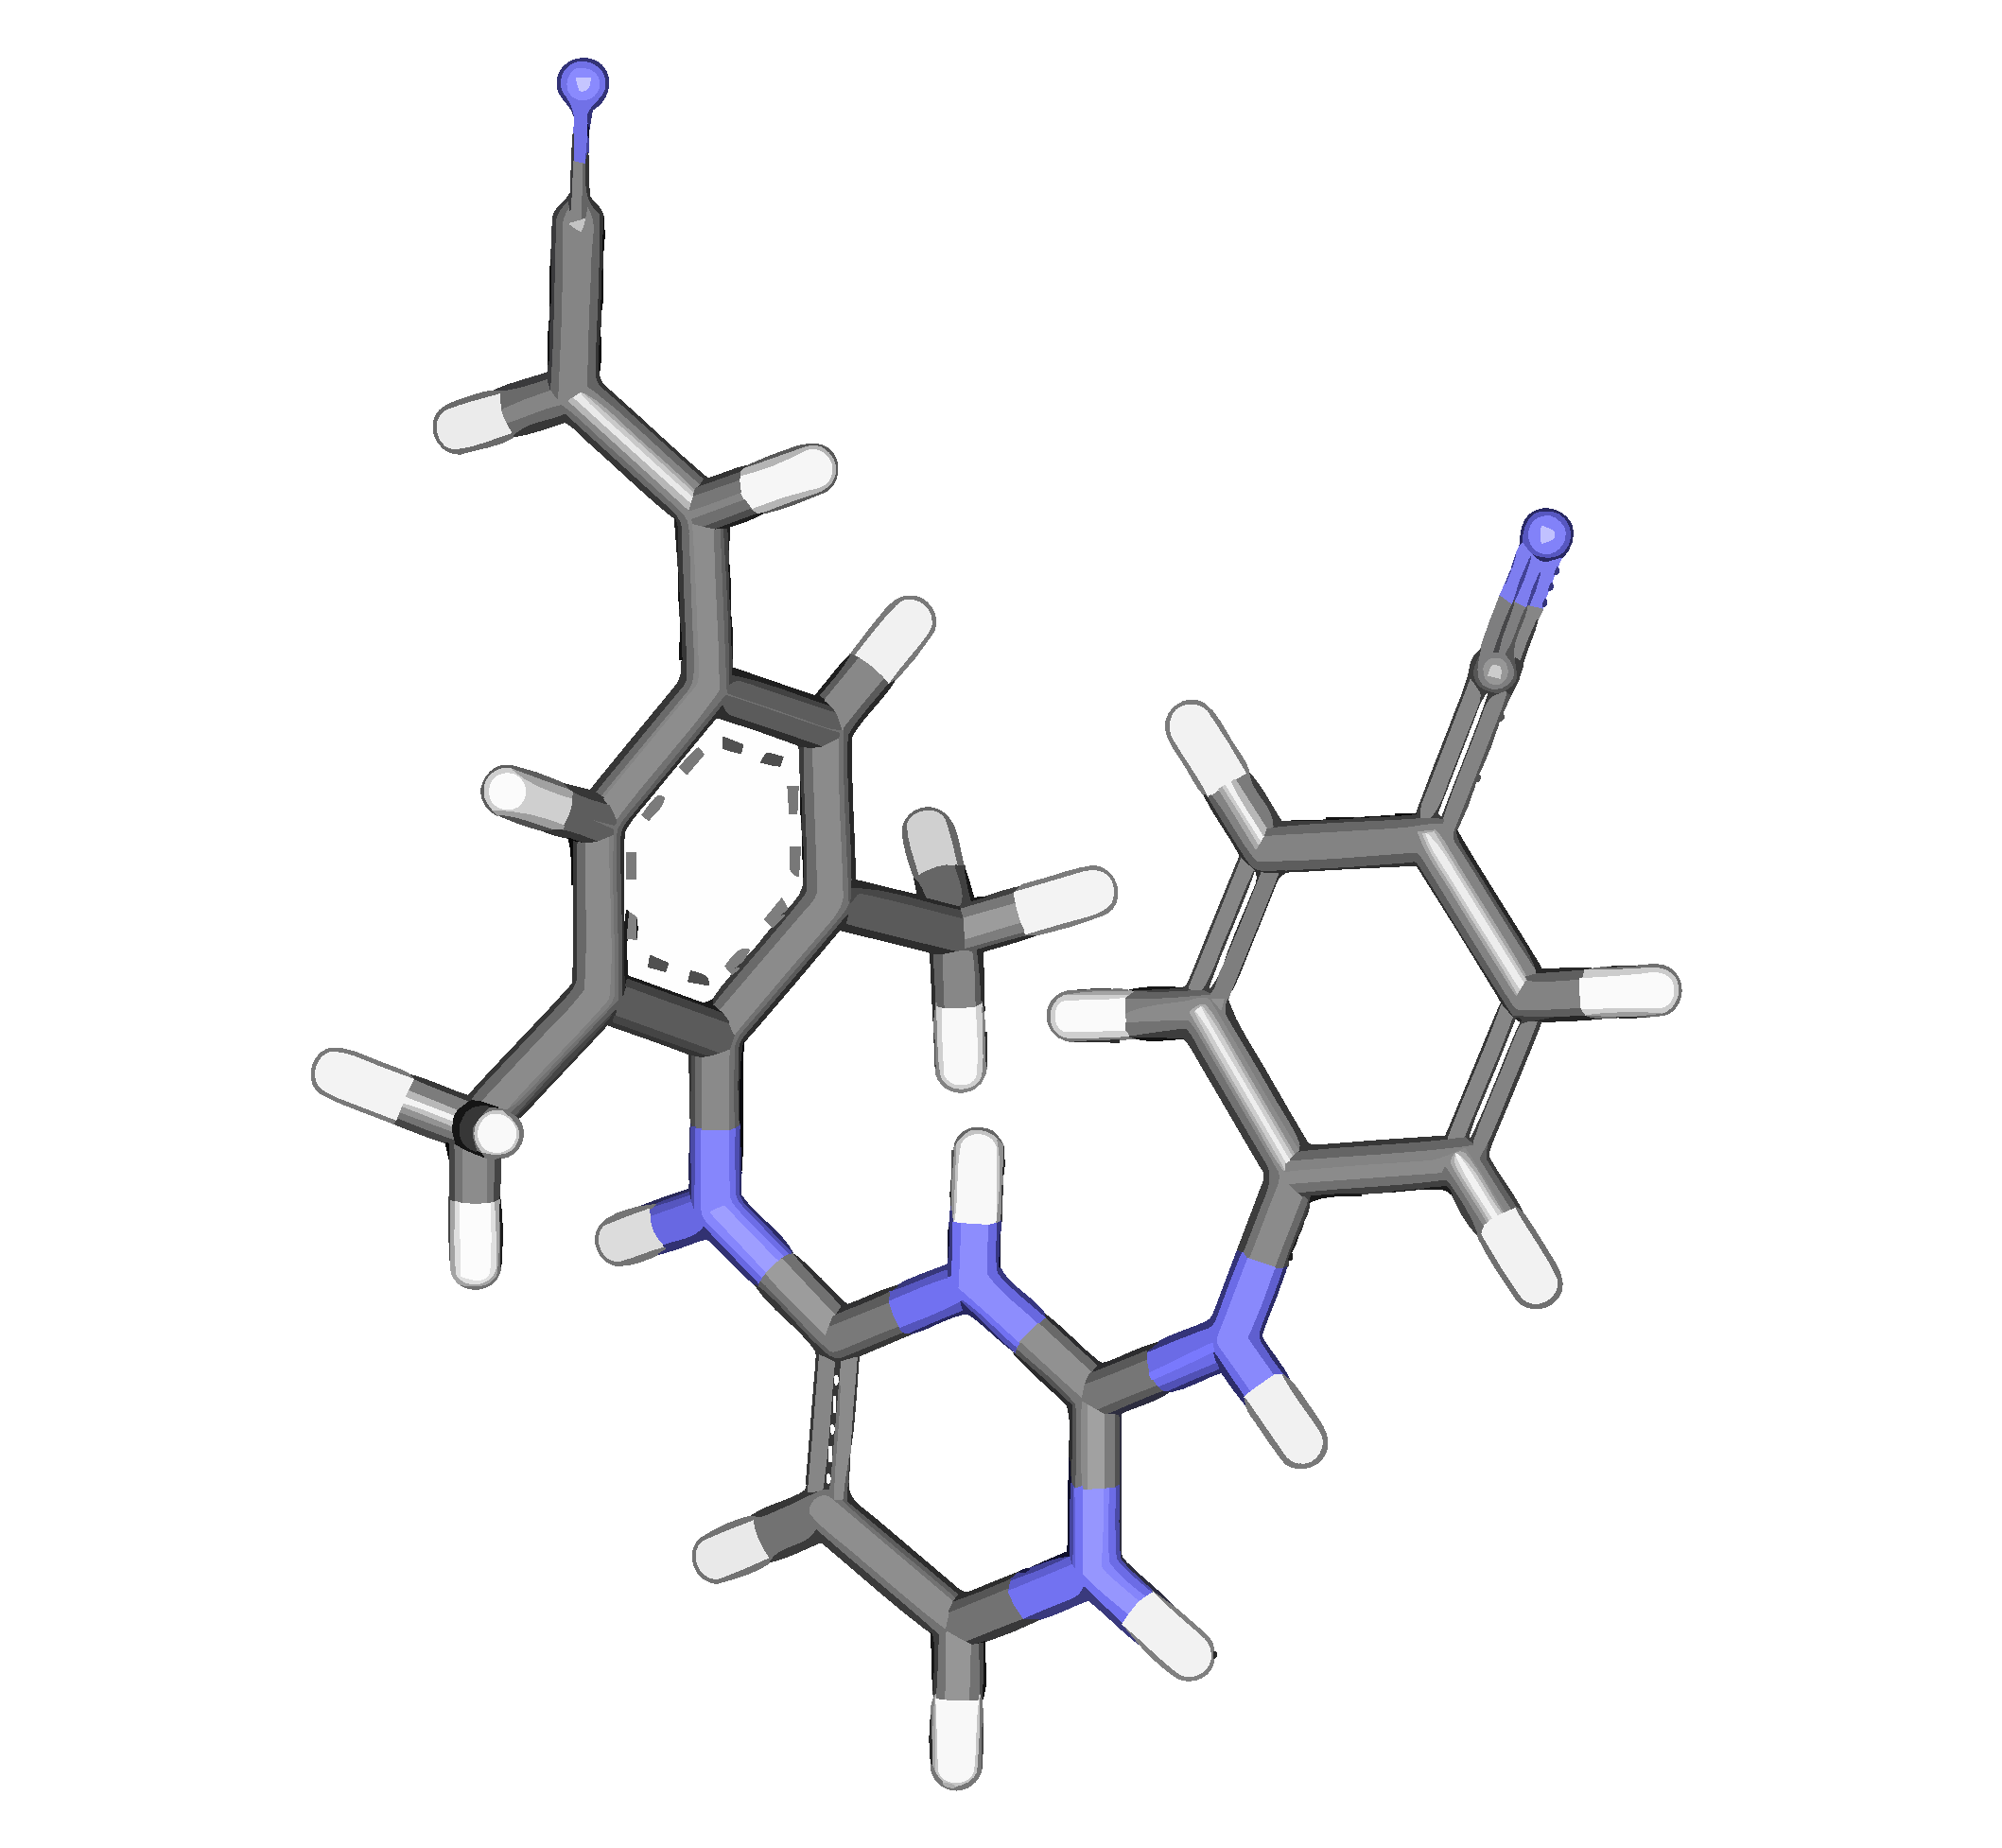
\includegraphics[width=0.11\linewidth]{Figures/Ligands/T27.eps}
}
\subfloat[4DX]
{
  \label{subfig:Ligands-4DX}
  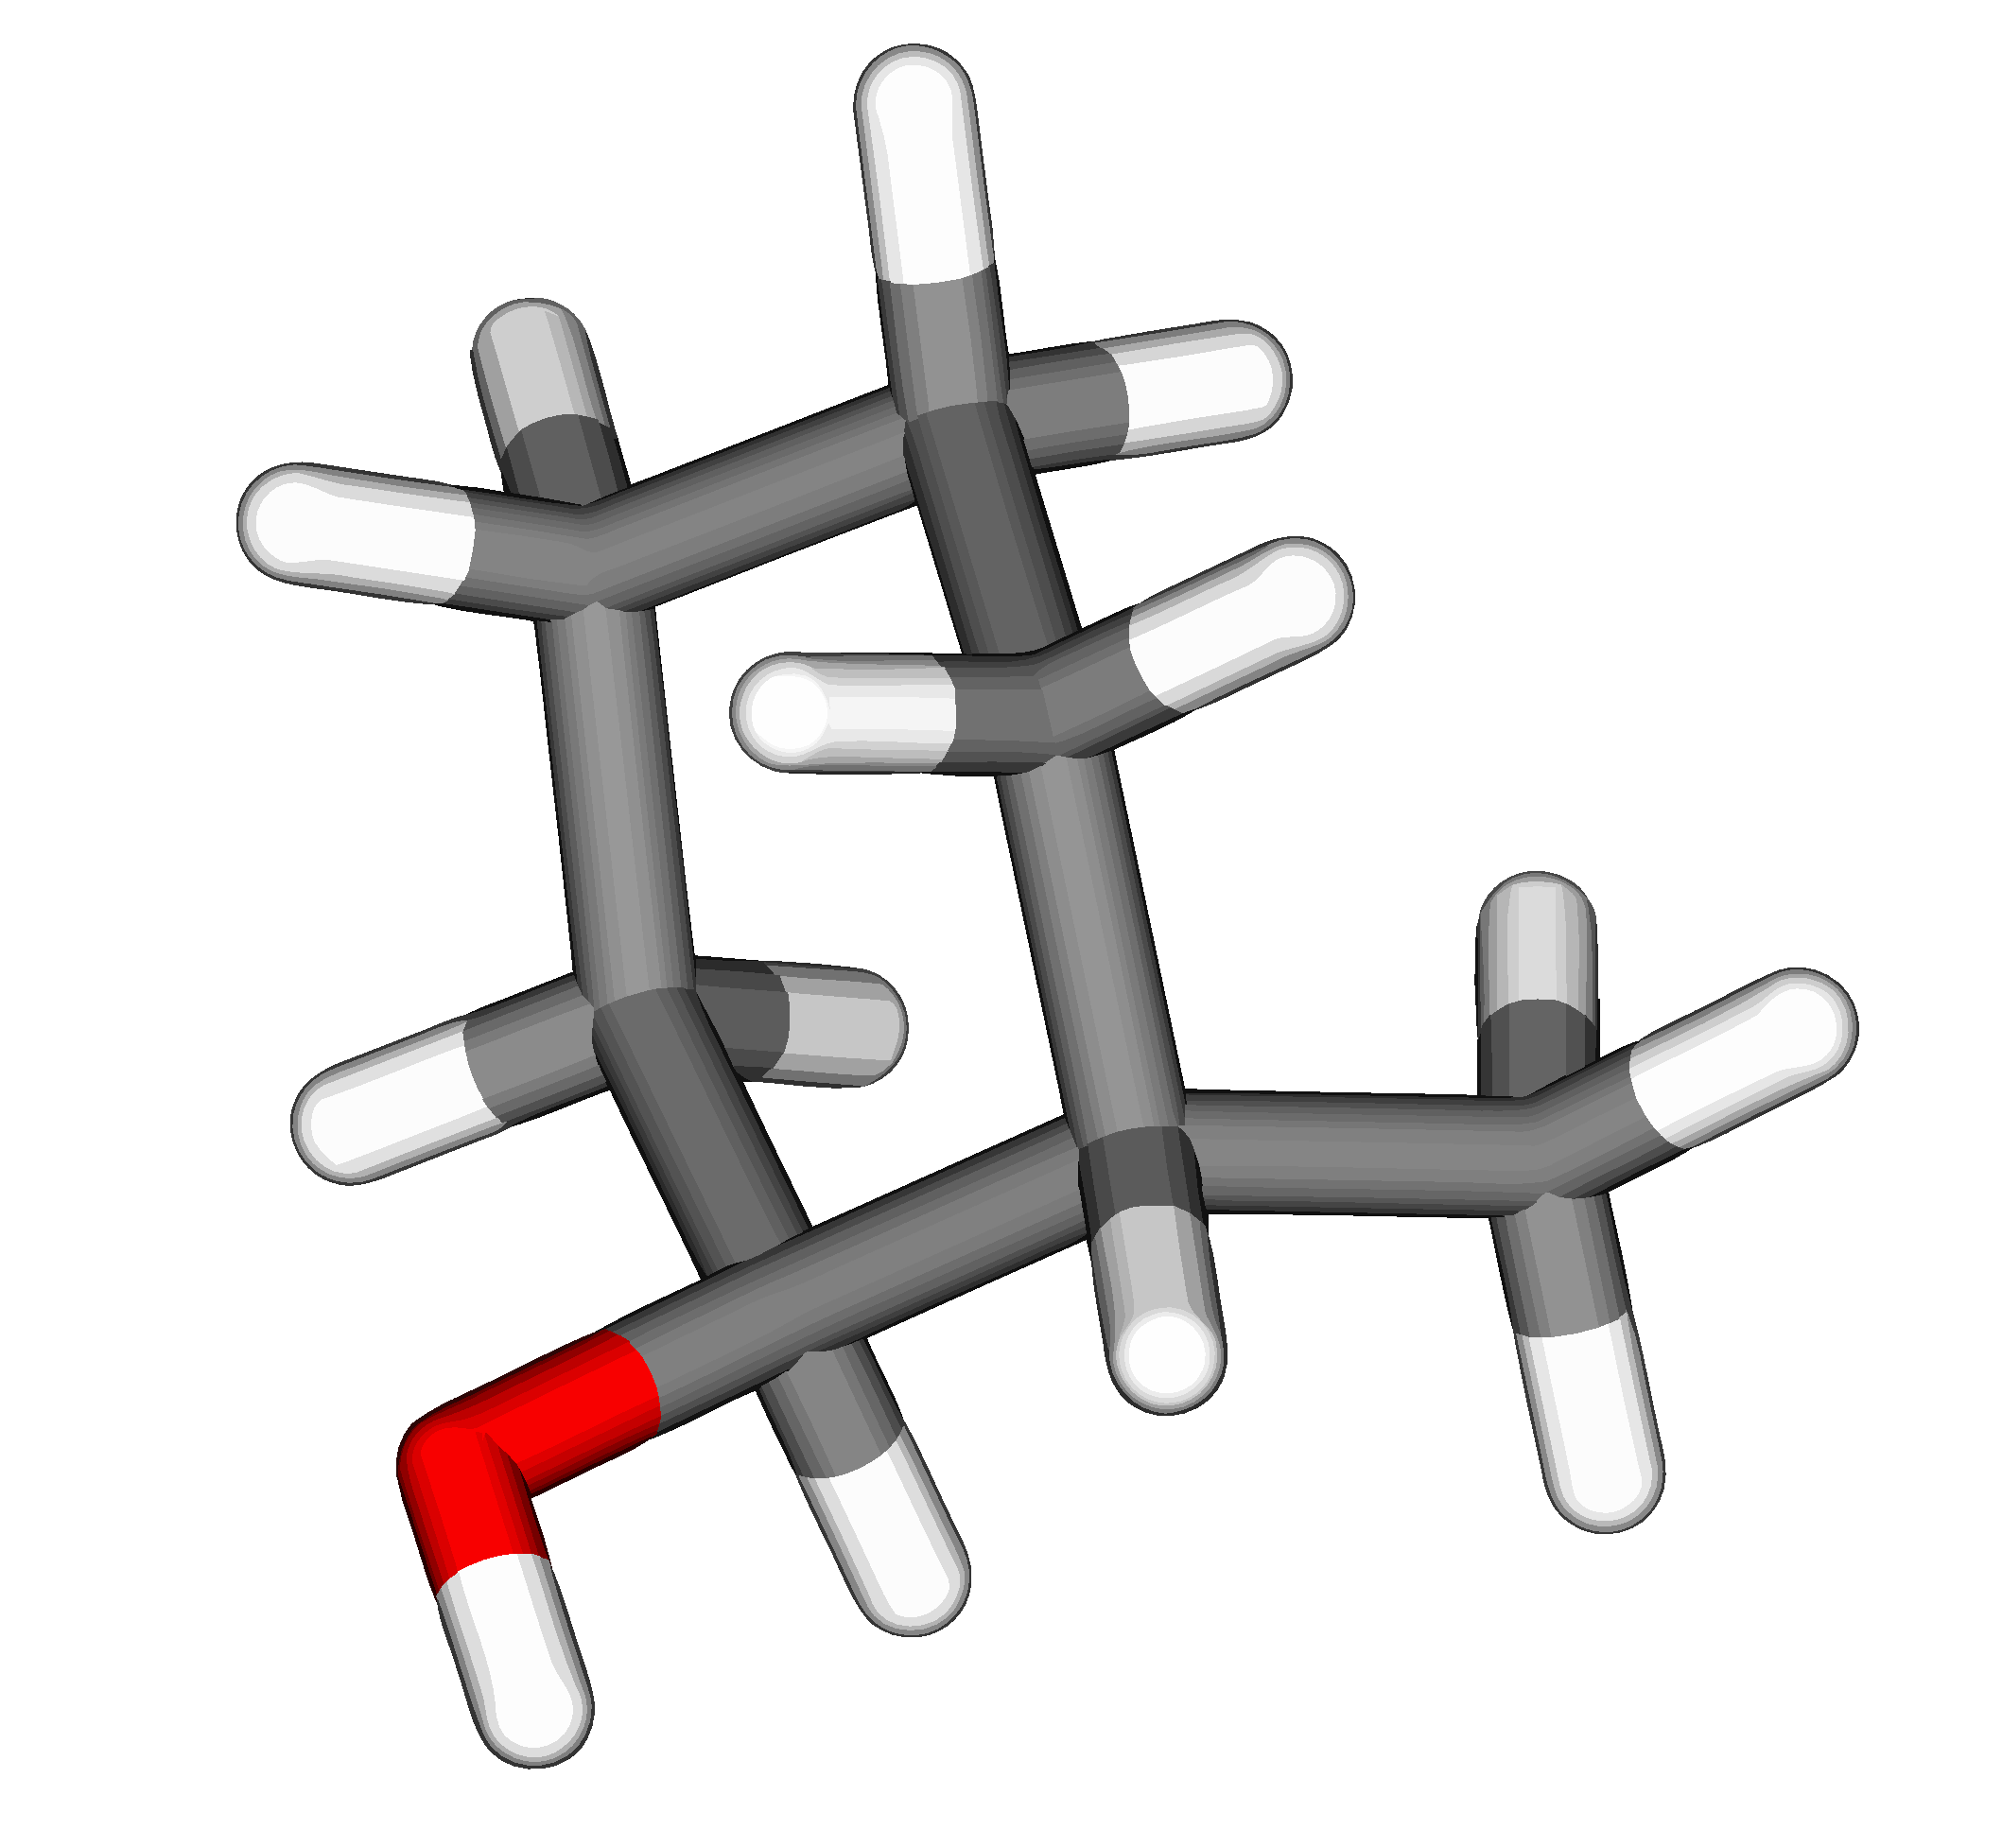
\includegraphics[width=0.11\linewidth]{Figures/Ligands/4DX.eps}
}
\subfloat[ZINC01019824]
{
  \label{subfig:Ligands-ZINC01019824}
  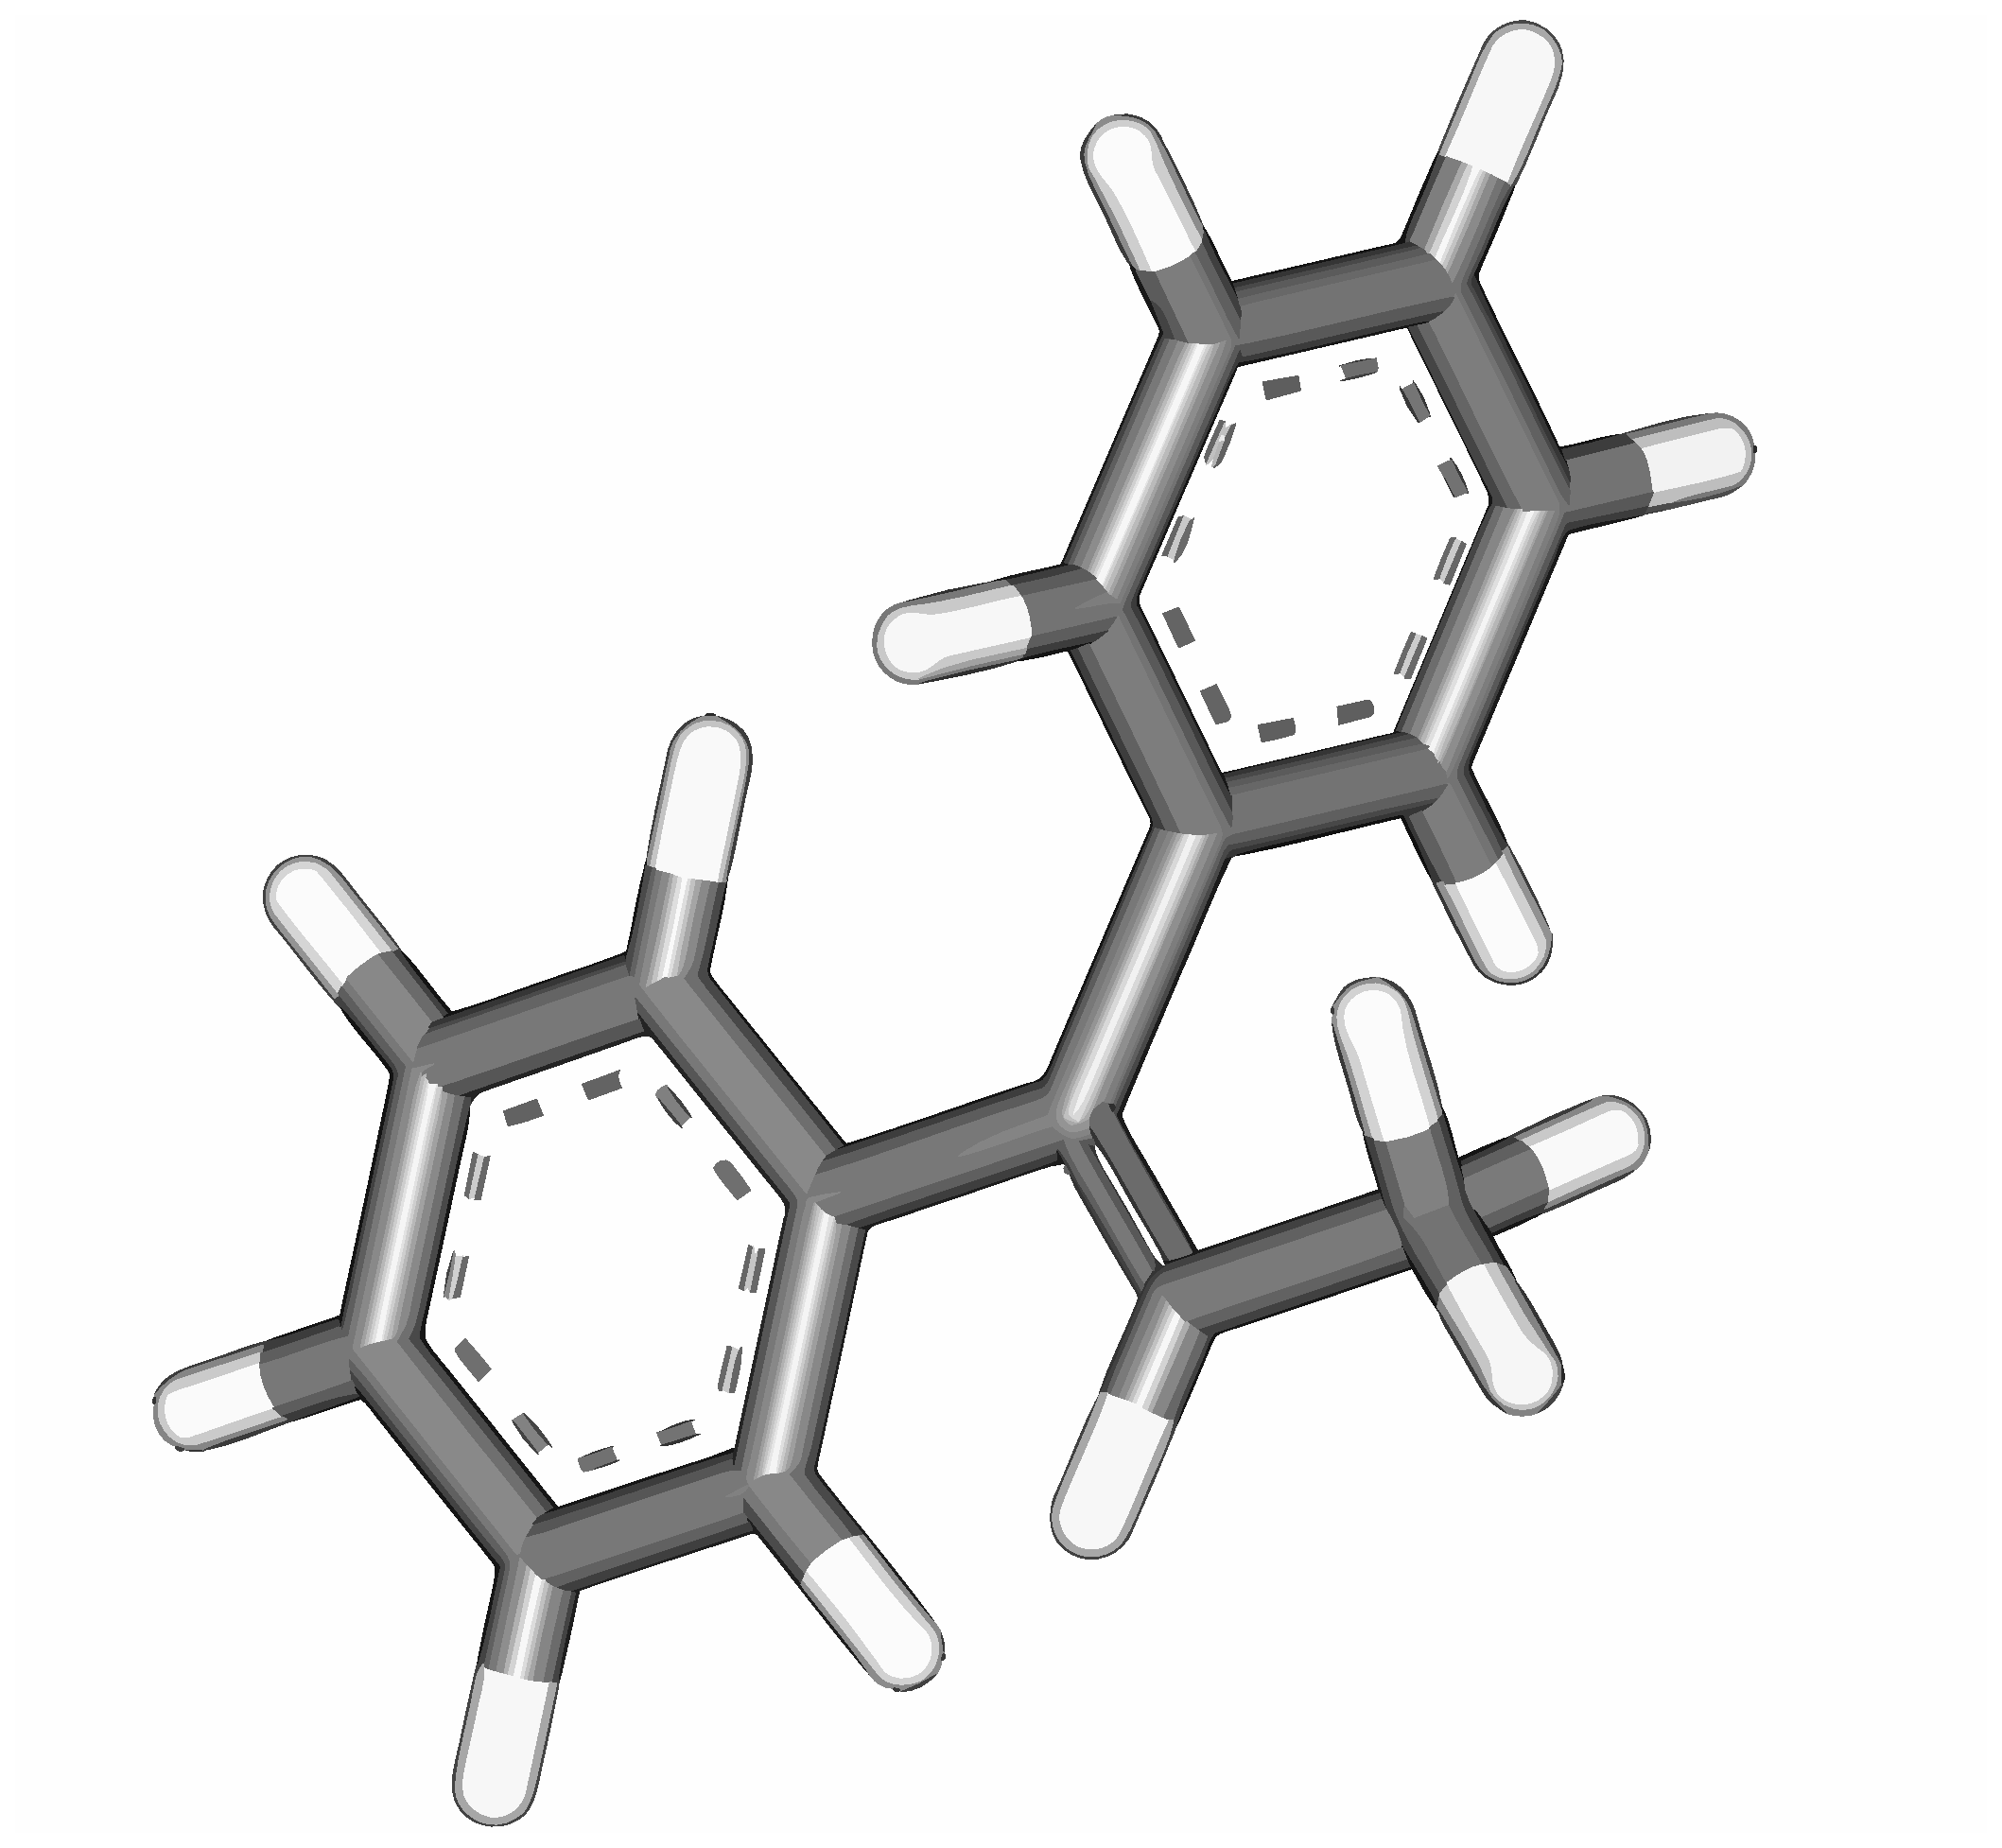
\includegraphics[width=0.11\linewidth]{Figures/Ligands/ZINC01019824.eps}
}
\subfloat[ZINC08442219]
{
  \label{subfig:Ligands-ZINC08442219}
  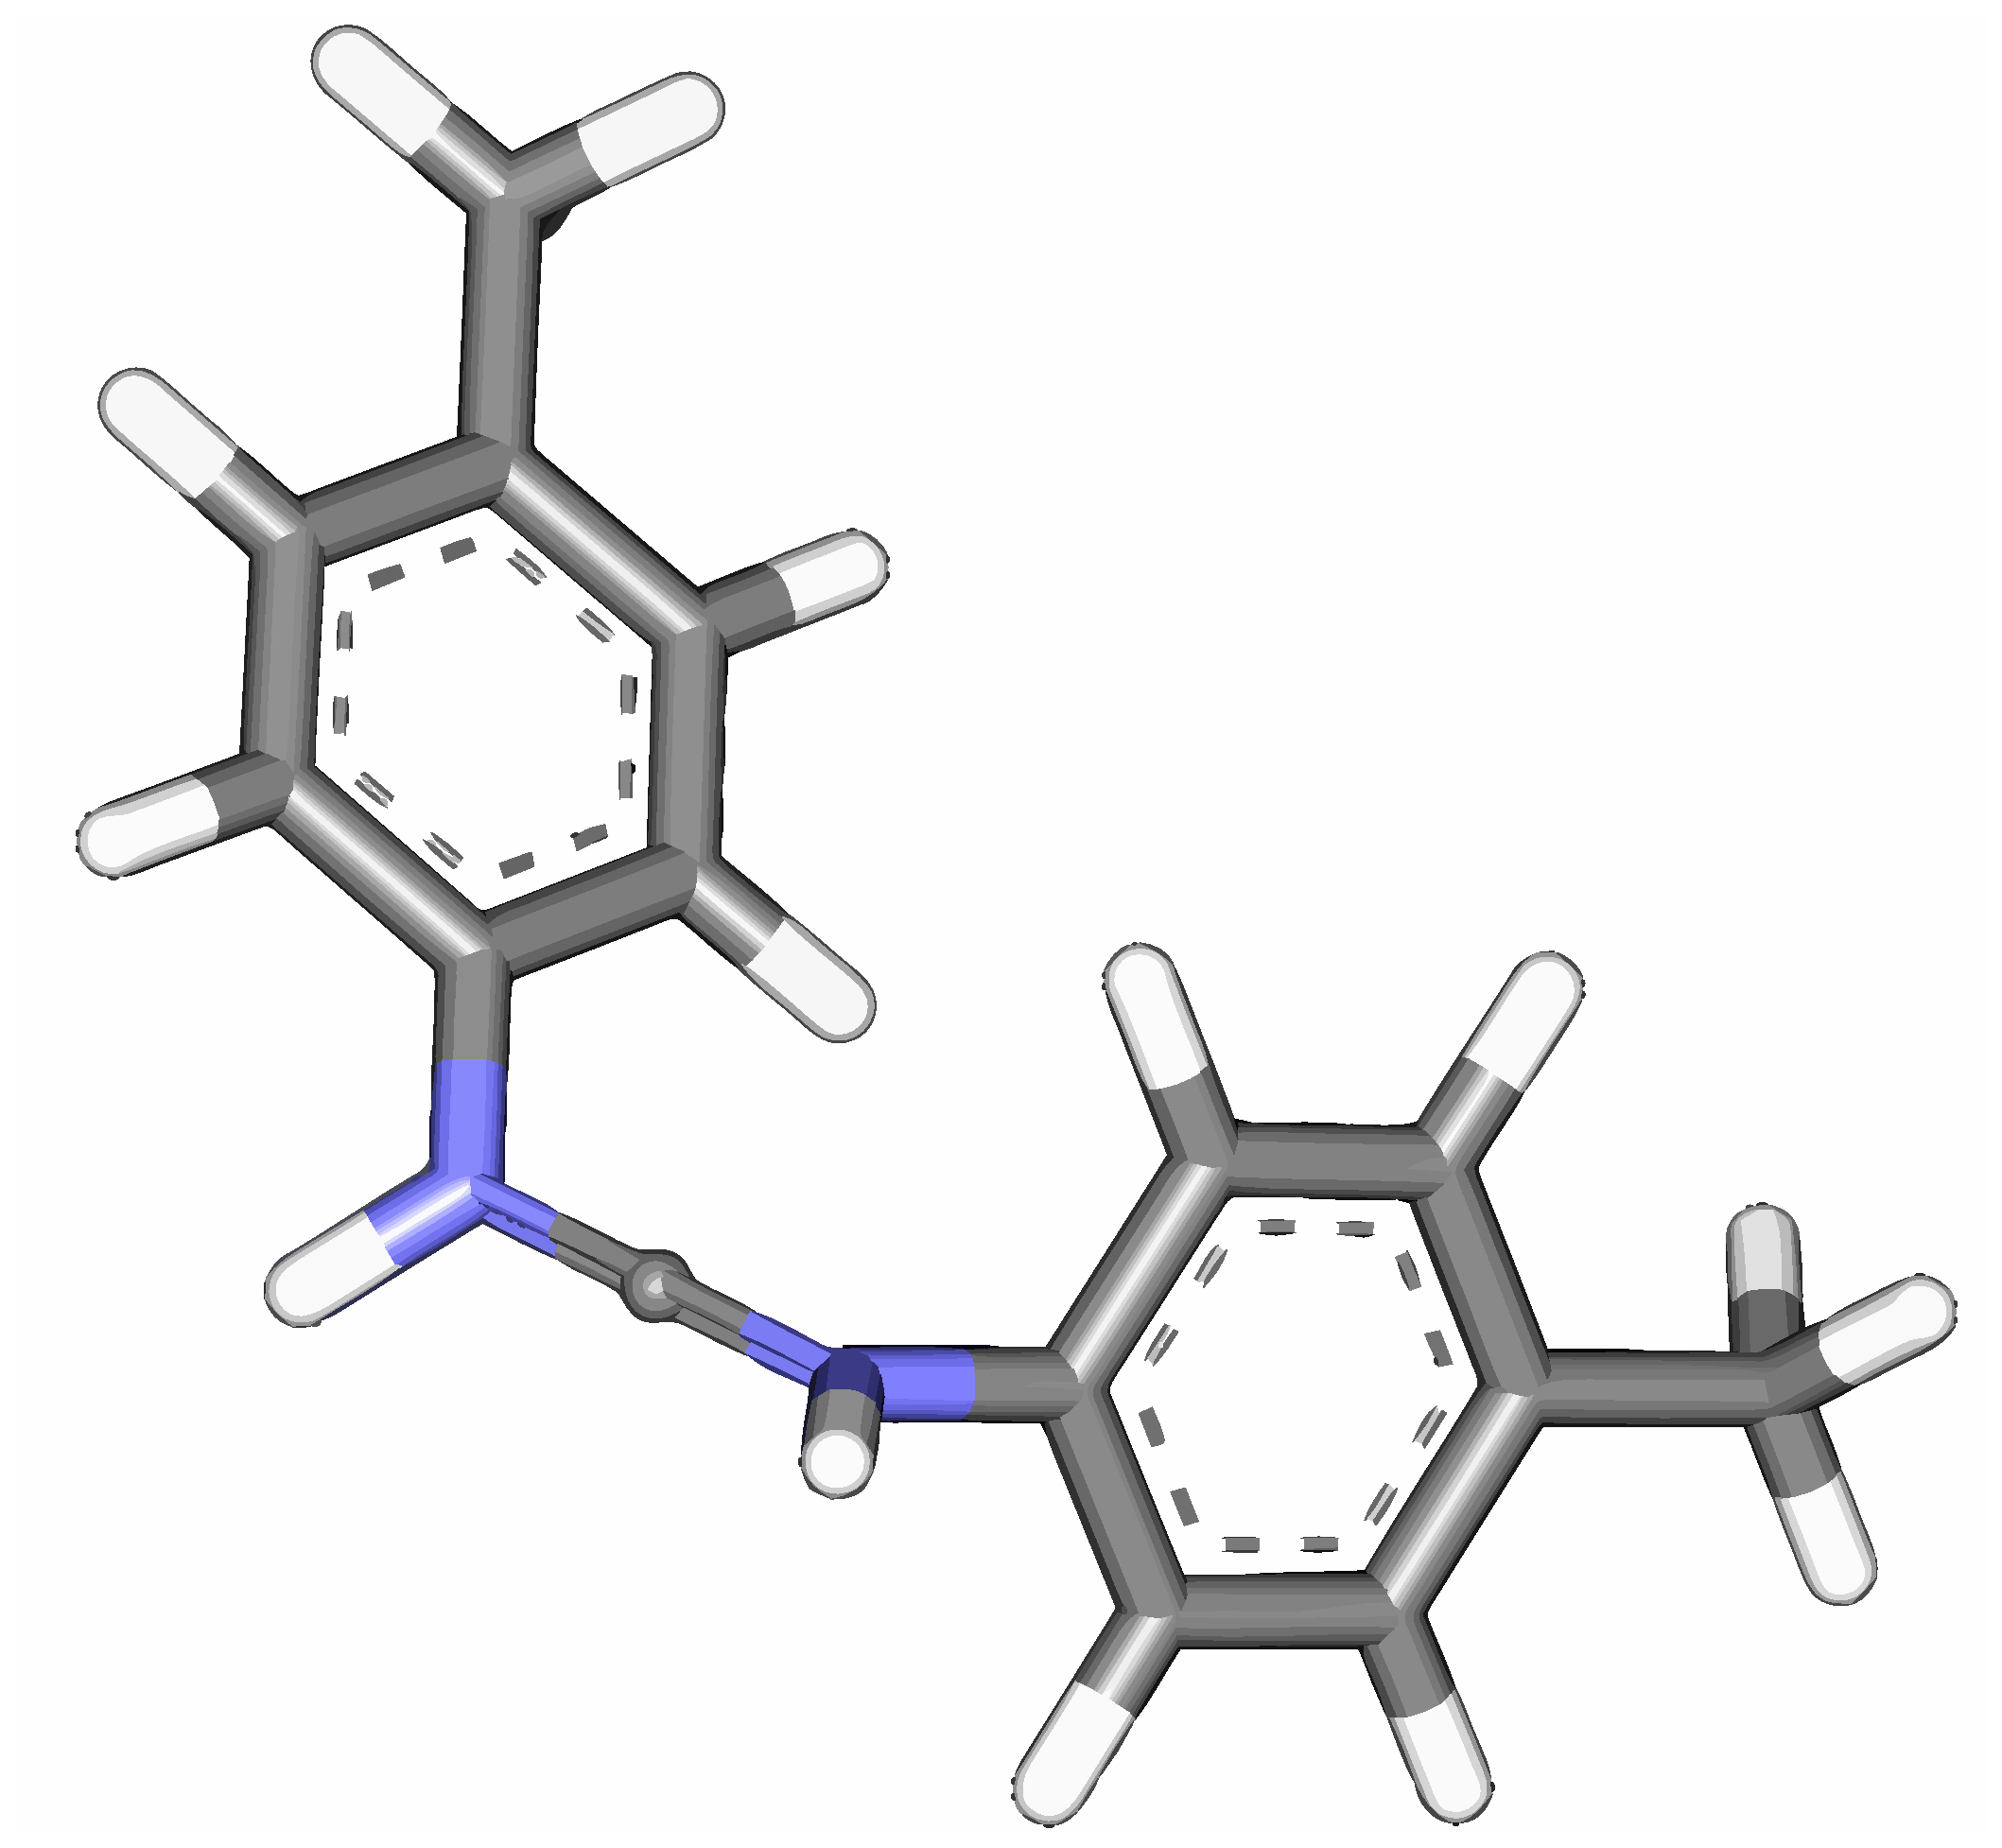
\includegraphics[width=0.11\linewidth]{Figures/Ligands/ZINC08442219.eps}
}
\subfloat[ZINC09365179]
{
  \label{subfig:Ligands-ZINC09365179}
  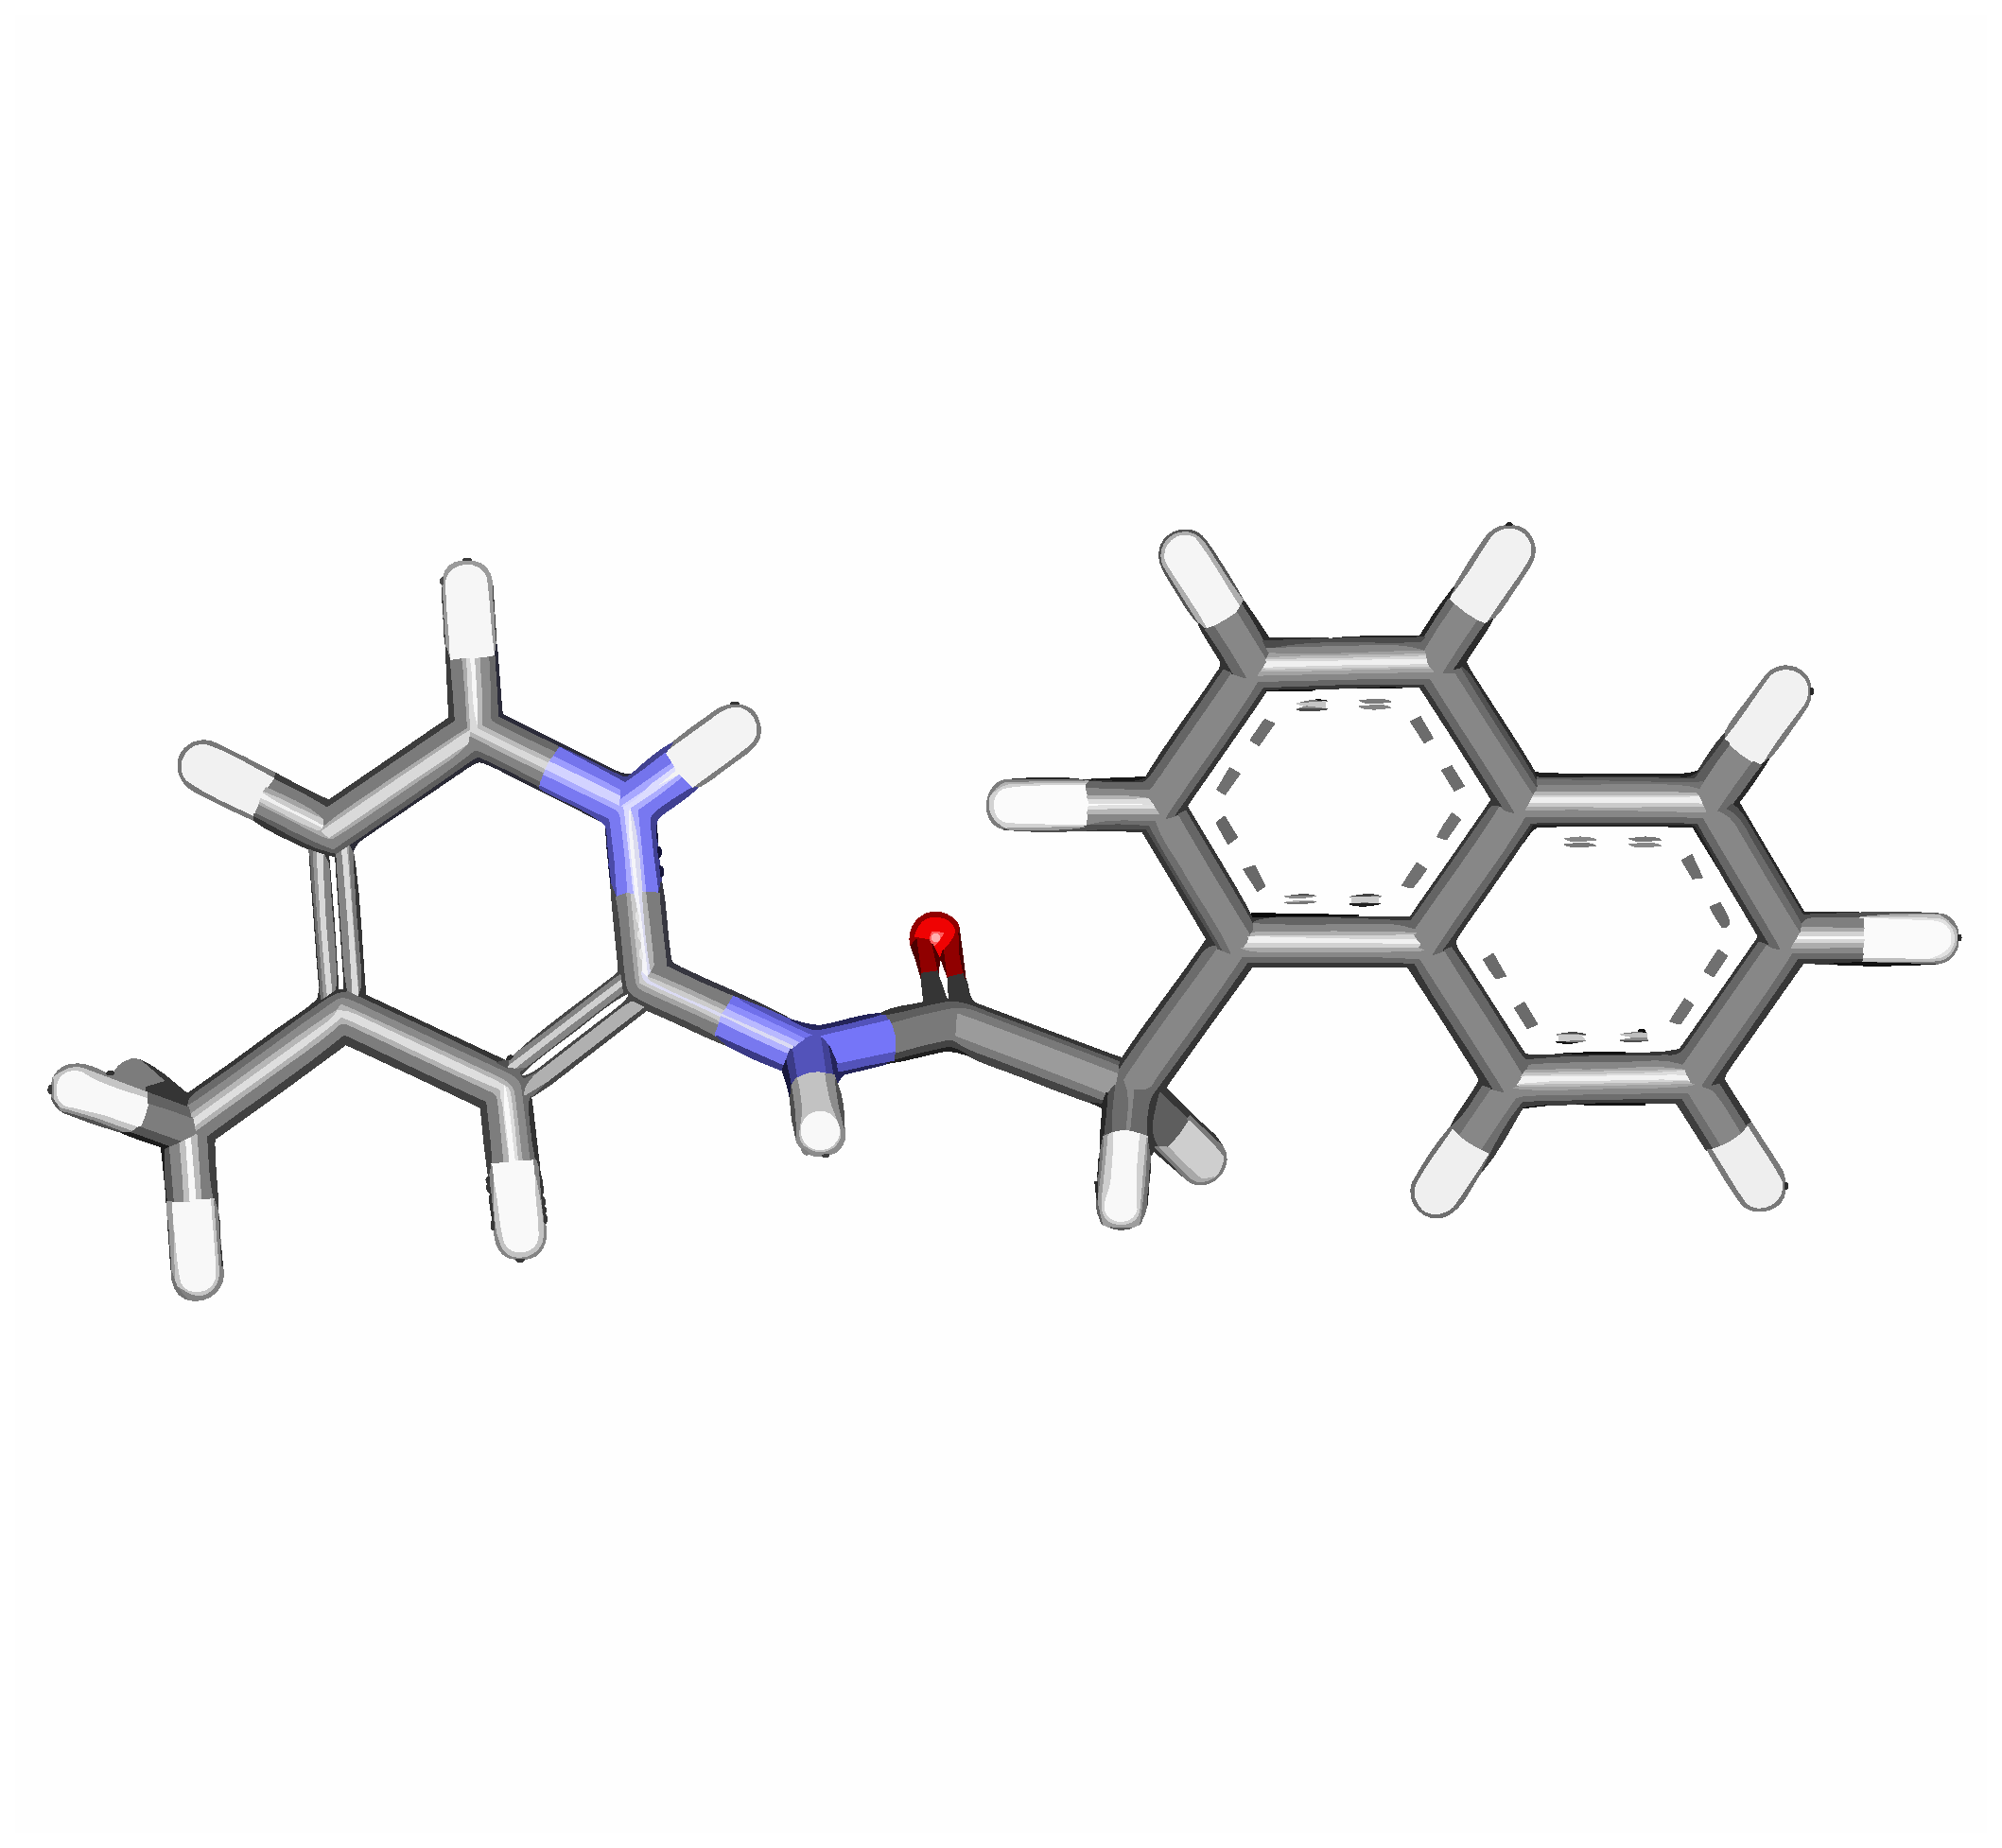
\includegraphics[width=0.11\linewidth]{Figures/Ligands/ZINC09365179.eps}
}
\subfloat[ZINC18153302]
{
  \label{subfig:Ligands-ZINC18153302}
  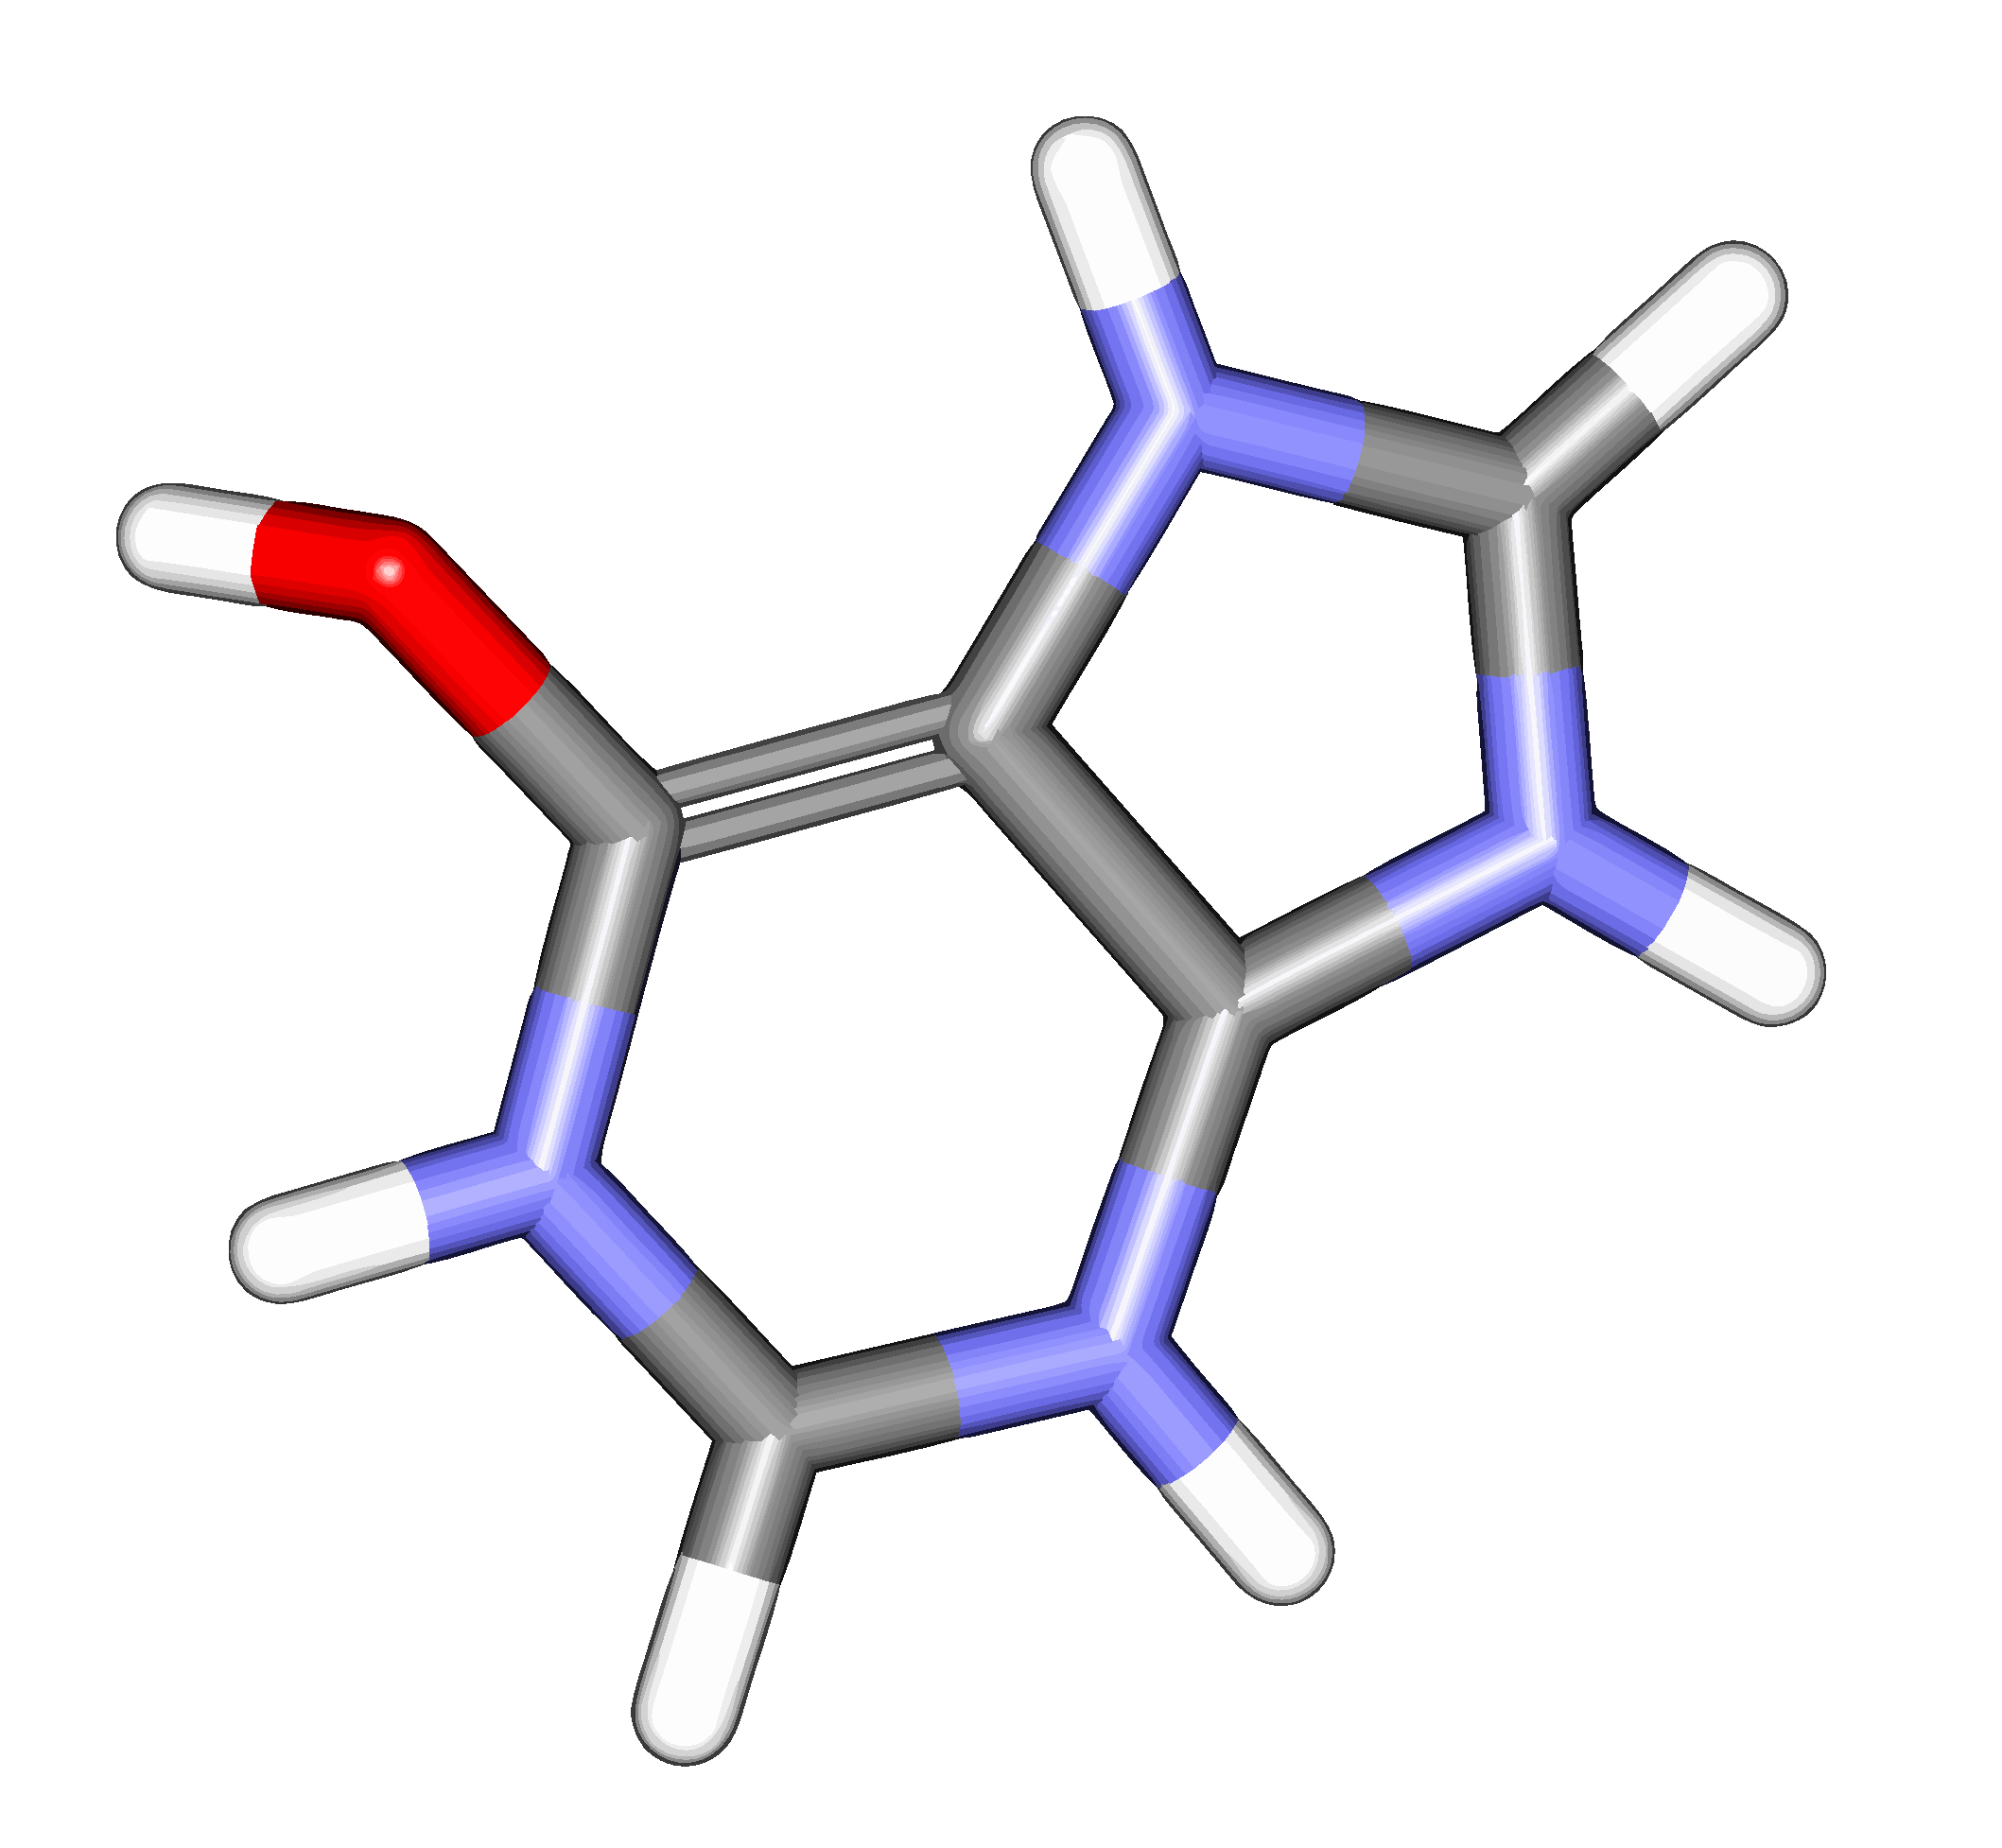
\includegraphics[width=0.11\linewidth]{Figures/Ligands/ZINC18153302.eps}
}
\subfloat[ZINC20030231]
{
  \label{subfig:Ligands-ZINC20030231}
  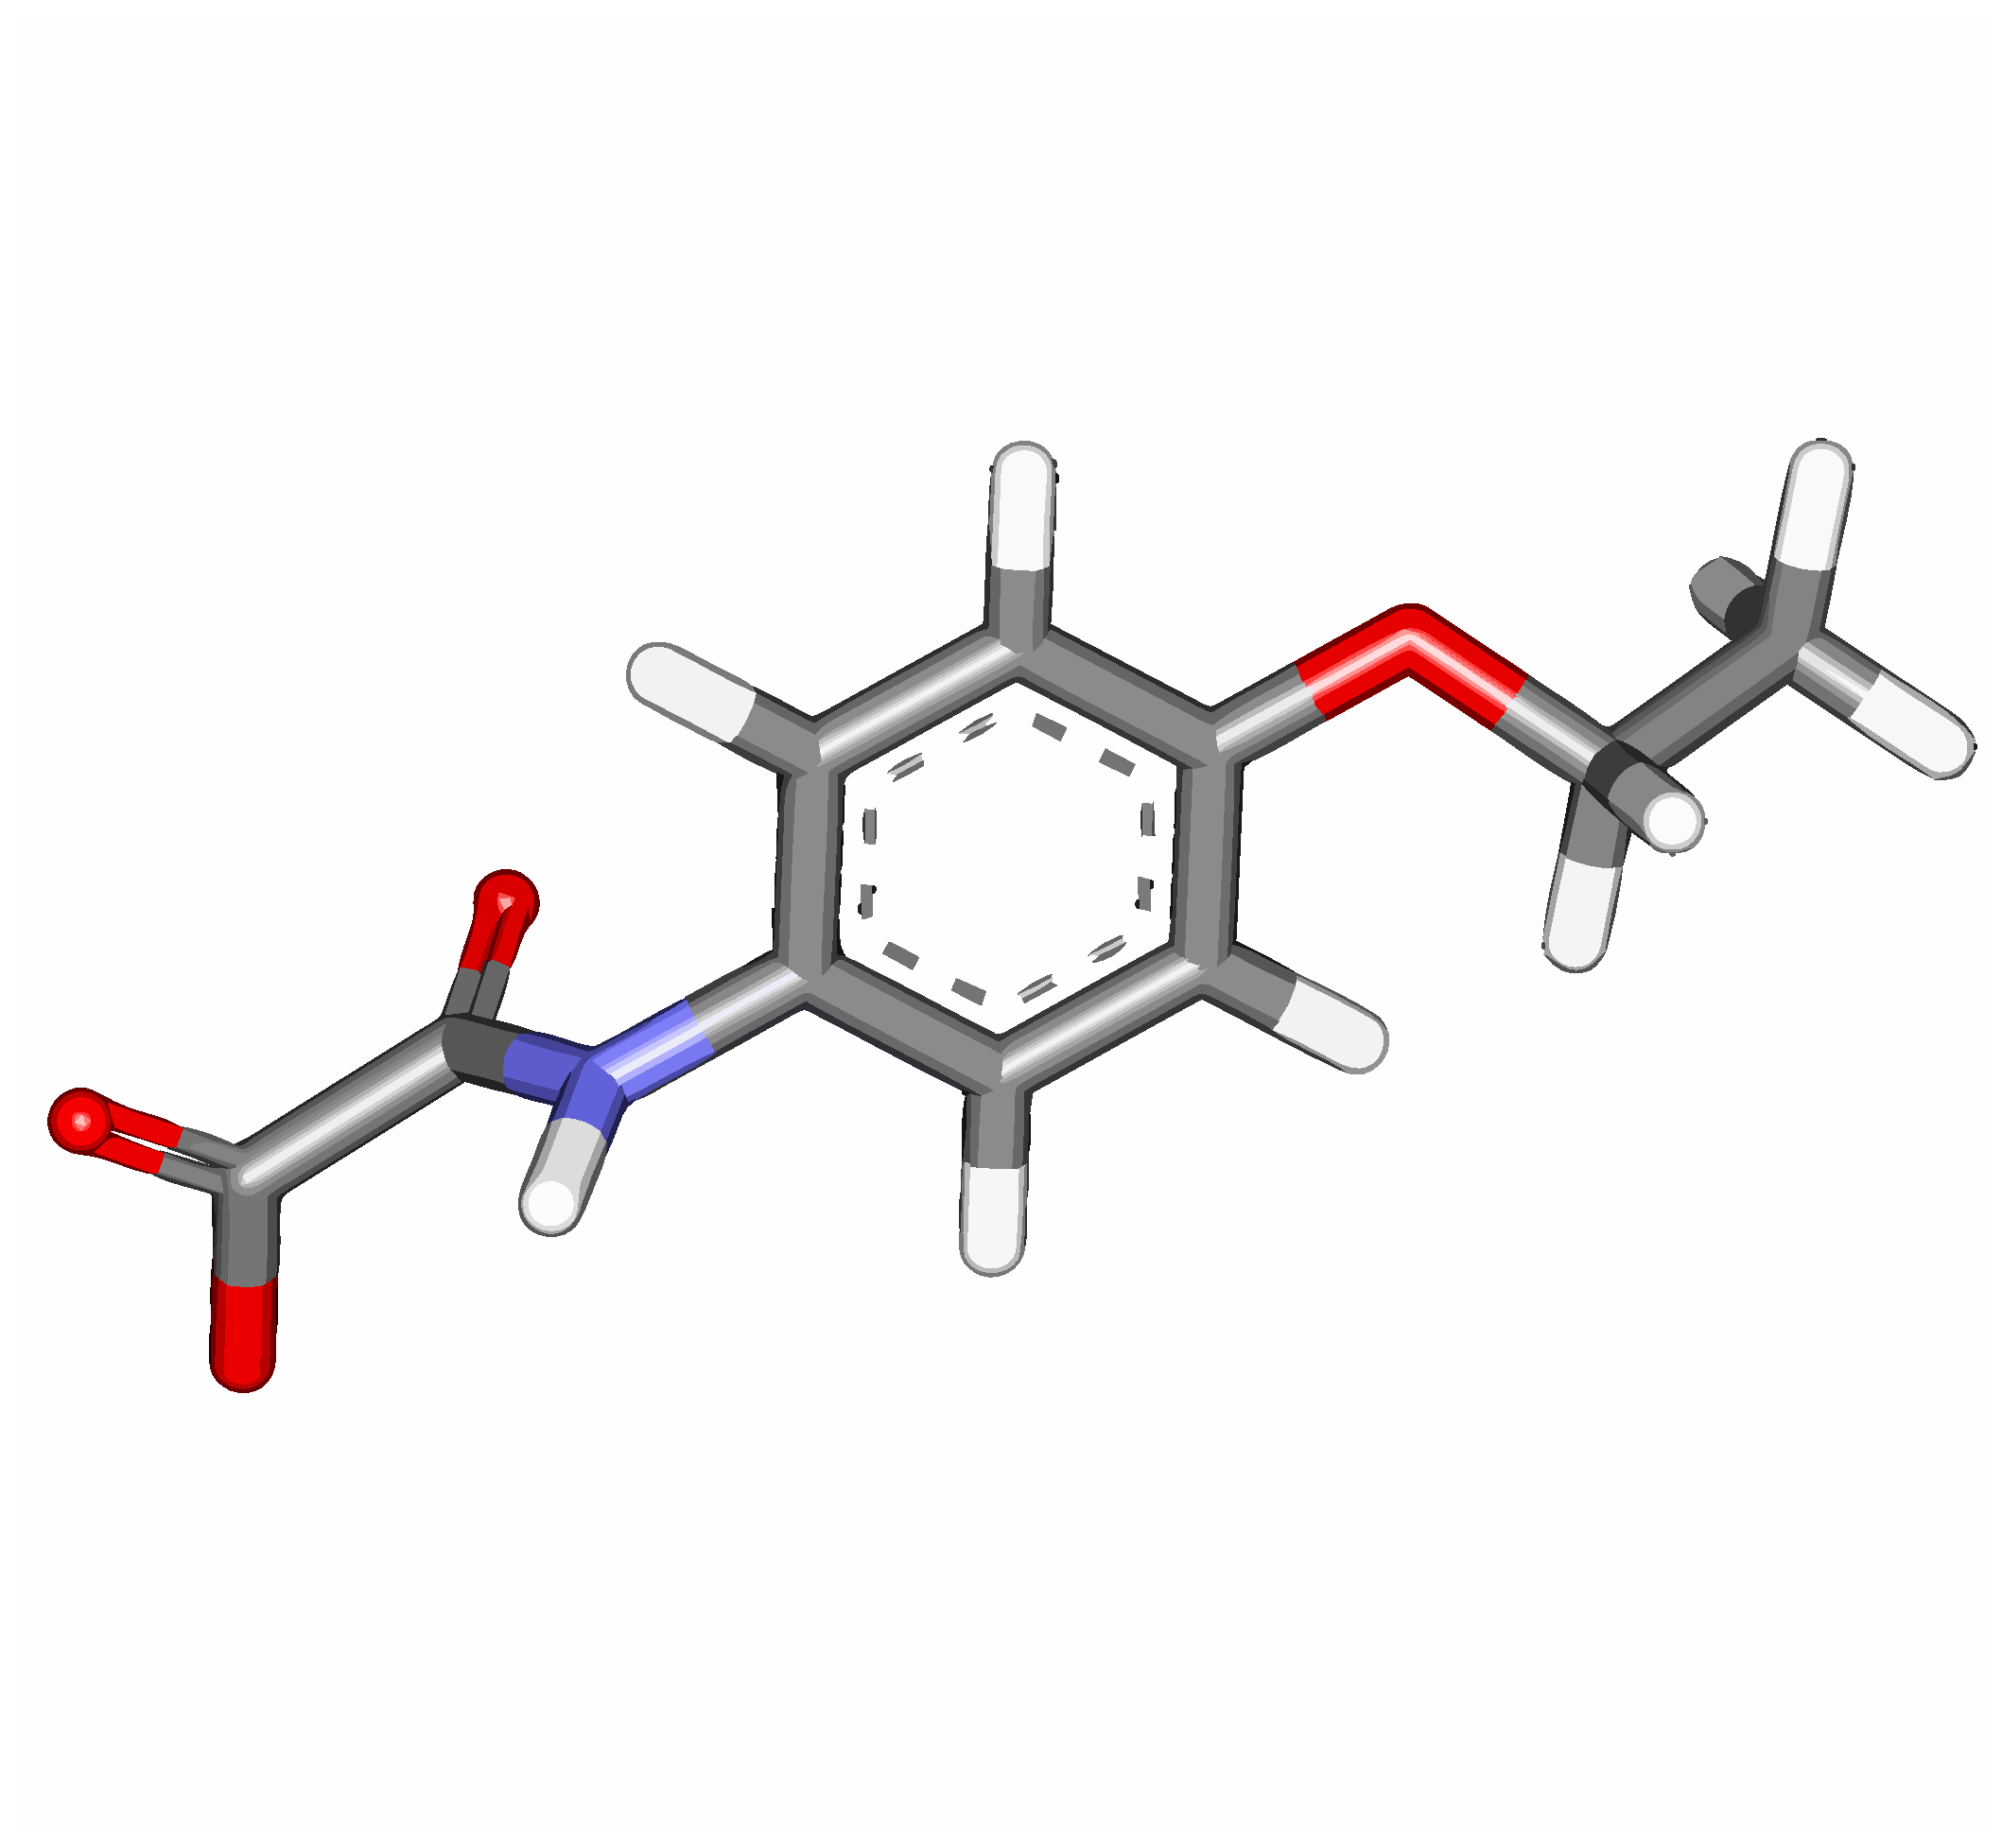
\includegraphics[width=0.11\linewidth]{Figures/Ligands/ZINC20030231.eps}
}
\caption{Stick representations and molecular weights of the 8 unique initial ligands.}
\label{fig:UniqueInitialLigands}
\end{figure*}

Phosphorus is a very common chemical element found in drugs. However, AutoGrow does not natively support phosphorus. Its bond length library does not include phosphorus, so it must rely on PDB CONECT records to detect covalent bonds. In contrast, igrow has built-in support for phosphorus. Its source code incorporates bond lengths for phosphorus, so it can recover covalent bonds from PDB ATOM/HETATM records. To test such capability, we picked an additional phosphorus-containing ligand named TFO from PDB, and generated ligands from TFO docking to HIV reverse transcriptase. The input ligand file consists of ATOM records only.

\subsection{Fragment Library}

Ligands are mutated by appending new fragments from a fragment library. There are two fragment libraries that accompanied with the release of AutoGrow, namely the small-fragment and the large-fragment libraries. We tested both libraries internally, and noticed early convergence when using the large-fragment library, which was quite problematic for testing purposes. So we focused on the small-fragment library, which is made up of 46 fragments. They are small in size, having 3 to 15 atoms and an average of 9.6 atoms with a standard deviation of 2.8 \cite{114}.

\section{Results}

We tested igrow v1.14 and compared it with AutoGrow 2.0.4, the most recent versions of both programs at the moment this paper was composed. The parameter settings for AutoGrow and igrow are listed in table \ref{tab:ParameterSettings}. The default values for AutoGrow were retained, i.e. 10, 20, 20, and 8 for the number of elitists, children, mutants, and generations, respectively.

The maximum number of atoms was set to 80 because we noticed from initial trials that the generated ligands of final generation consisted of around 70 atoms but their molecular weight already exceeded 500 Da.

To make a fair comparison, the settings for igrow were set to be identical to AutoGrow.

\begin{table}
\centering
\begin{tabular*}
{\linewidth}
{@{\extracolsep{\fill}}lrr}
\noalign{\smallskip}\toprule
Program & AutoGrow & igrow\\
\midrule
\noalign{\smallskip}
Number of elitists & 10 & 10\\
Number of children & 20 & 20\\
Number of mutants & 20 & 20\\
Number of generations & 8 & 24\\
Docking frequency & 1 & 3\\
Max number of atoms & 80 & 80\\
\bottomrule
\end{tabular*}
\caption{Parameter settings for AutoGrow and igrow. Elitists refer to the best ligands of a generation that will survive directly into the next generation. Children refer to ligands generated by crossover. Mutants refer to ligands generated by mutation.}
\label{tab:ParameterSettings}
\end{table}

So far we have collected 3 receptors, each of which is associated with 6 initial ligands. Therefore there are 18 test cases in total. Since genetic algorithm is stochastic, we ran AutoGrow and igrow for 9 times for each test case under the parameter settings shown in \ref{tab:ParameterSettings}, simultaneously on 6 Linux machines with Ubuntu 10.04.1 x86\_64, Dual Intel Xeon Quad Core 2.4GHz, and 32GB RAM. Each AutoGrow execution and igrow execution cost approximately 3 hours and 2.4 hours respectively on average.

\subsection{Binding Pose}

In order to validate the correctness of ligands generated by igrow, we picked out the best ligand from each test case and visualized it in complex of its corresponding receptor. Here, the best ligand refers to the one that have the lowest free energy.
Figure \ref{fig:BestLigands} demonstrates one particular test case.

\begin{figure*}[p]
\centering
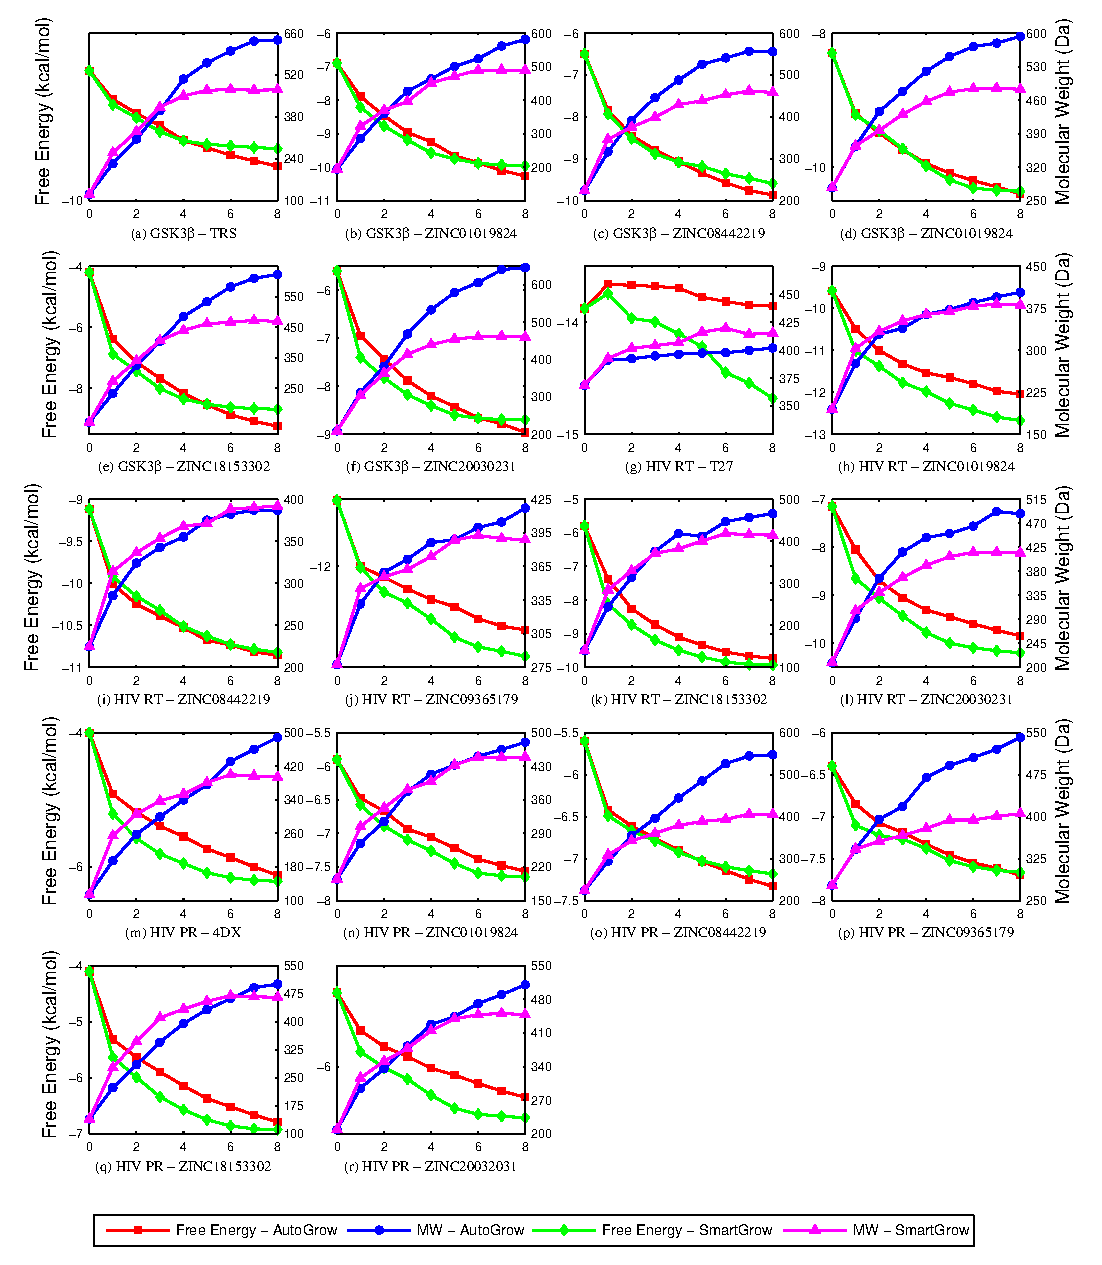
\includegraphics[width=1\linewidth]{Figures/Results/Best5.eps}
\caption{Average free energies and molecular weights of the best 5 ligands generated by AutoGrow and igrow of each generation. Generation 0 refers to the initial ligand. Blue circles: average free energies of the best 5 ligands generated by AutoGrow. Green diamonds: average free energies of the best 5 ligands generated by igrow. Red squares: average molecular weights of the best 5 ligands generated by AutoGrow. Purple triangles: average molecular weights of the best 5 ligands generated by igrow. First 6 initial ligands dock to glycogen synthase kinase 3 beta. Middle 6 initial ligands dock to HIV reverse transcriptase. Last 6 initial ligands dock to HIV protease.}
\label{fig:Best5}
\end{figure*}

\begin{figure*}
\centering
\subfloat[Initial ligand.]
{
  \label{subfig:1J1B-ZINC01019824}
  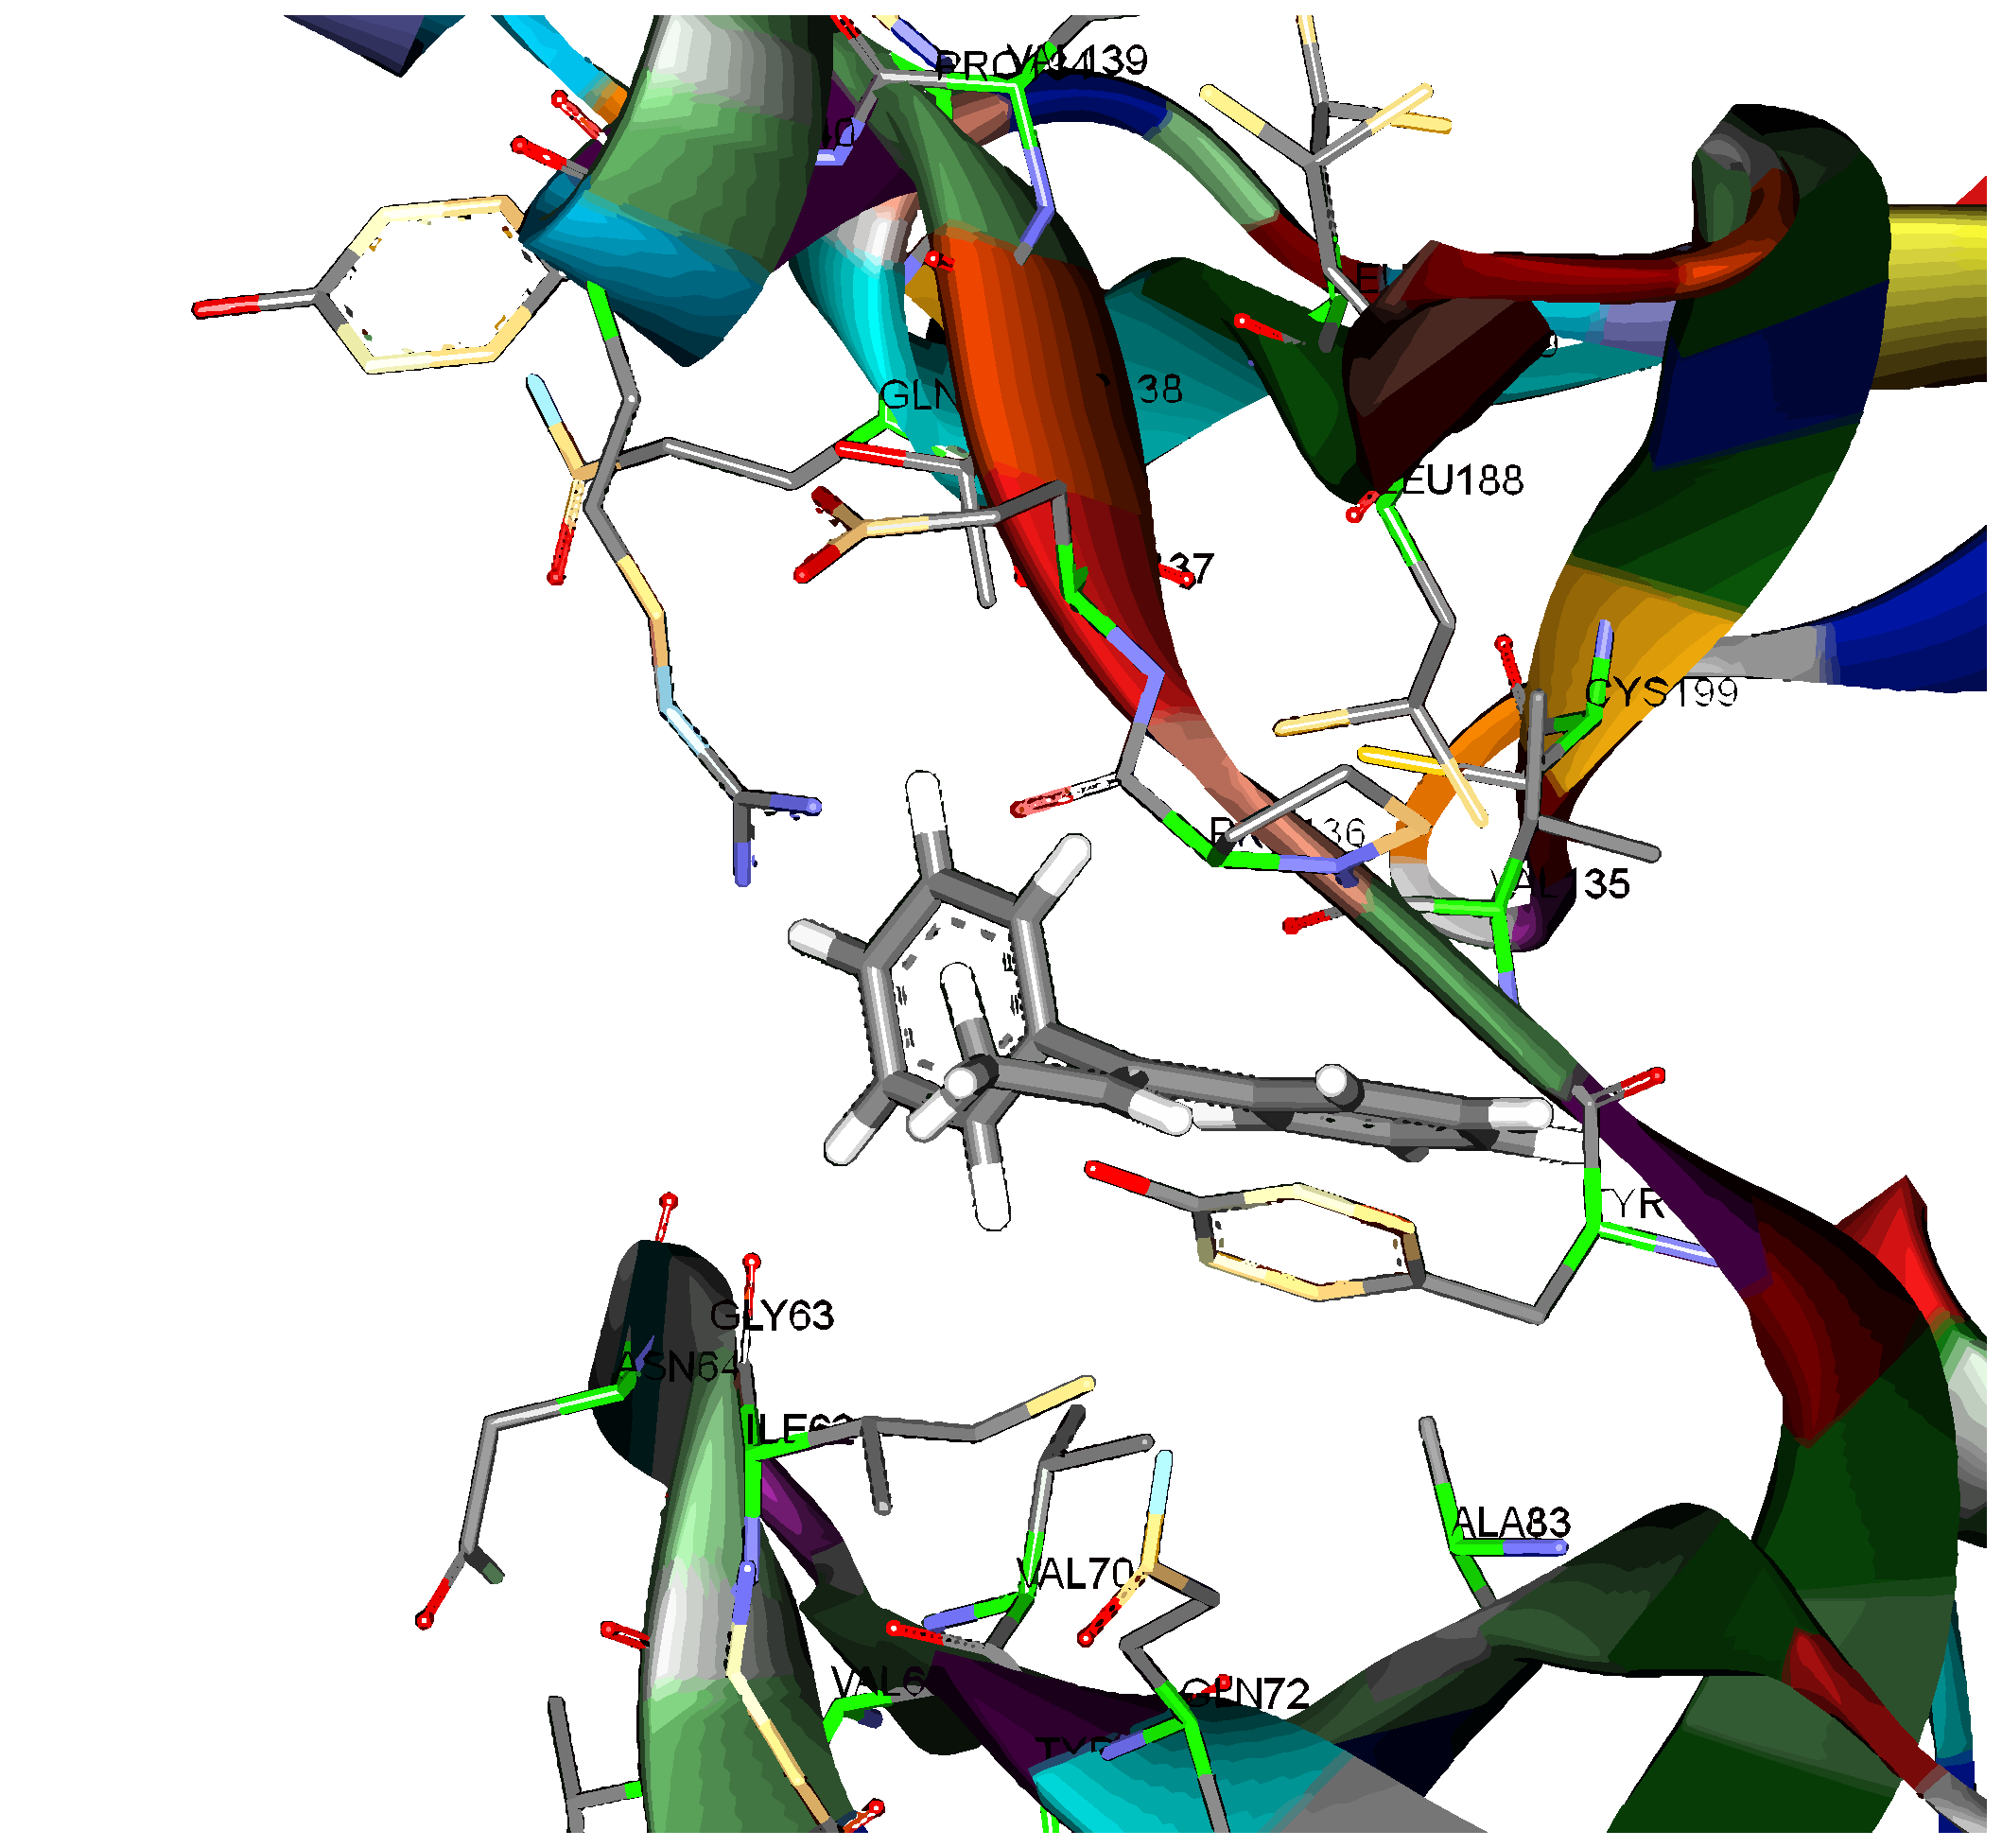
\includegraphics[width=0.31\linewidth]{Figures/Results/1J1B-ZINC01019824.eps}
}
\subfloat[The best ligand generated by AutoGrow.]
{
  \label{subfig:1J1B-ZINC01019824-AutoGrow}
  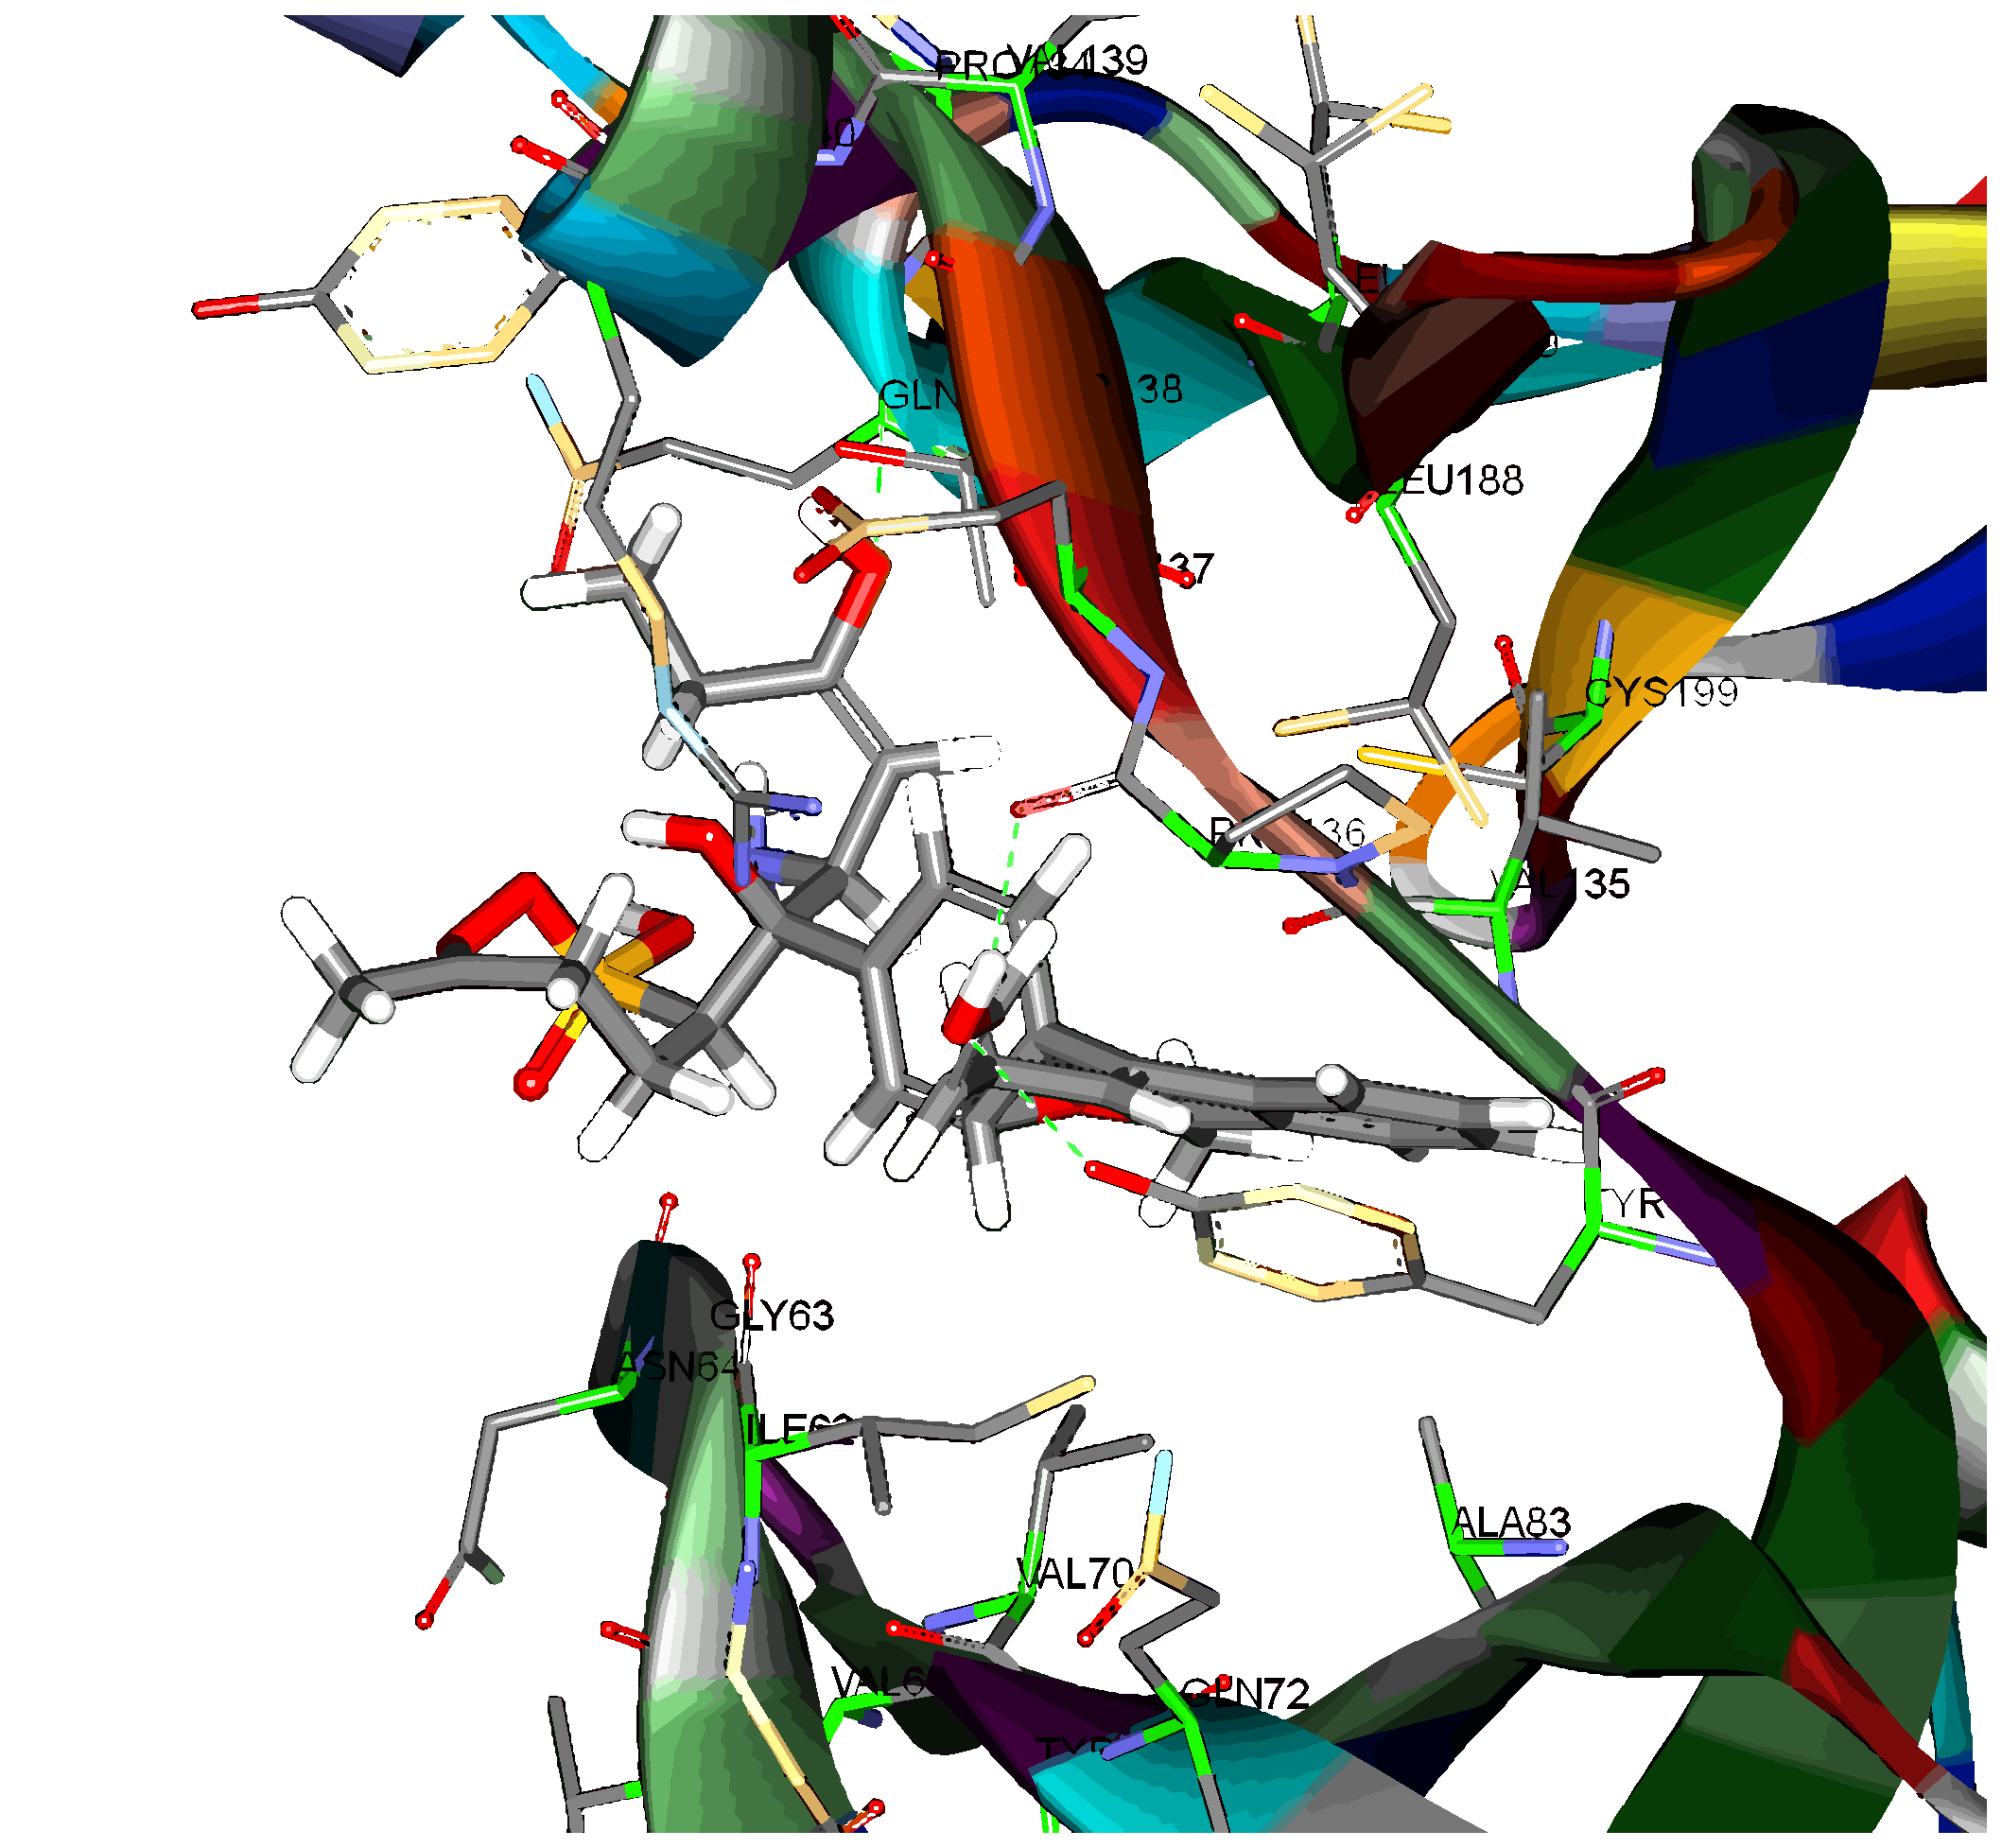
\includegraphics[width=0.31\linewidth]{Figures/Results/1J1B-ZINC01019824-AutoGrow.eps}
}
\subfloat[The best ligand generated by igrow.]
{
  \label{subfig:1J1B-ZINC01019824-igrow}
  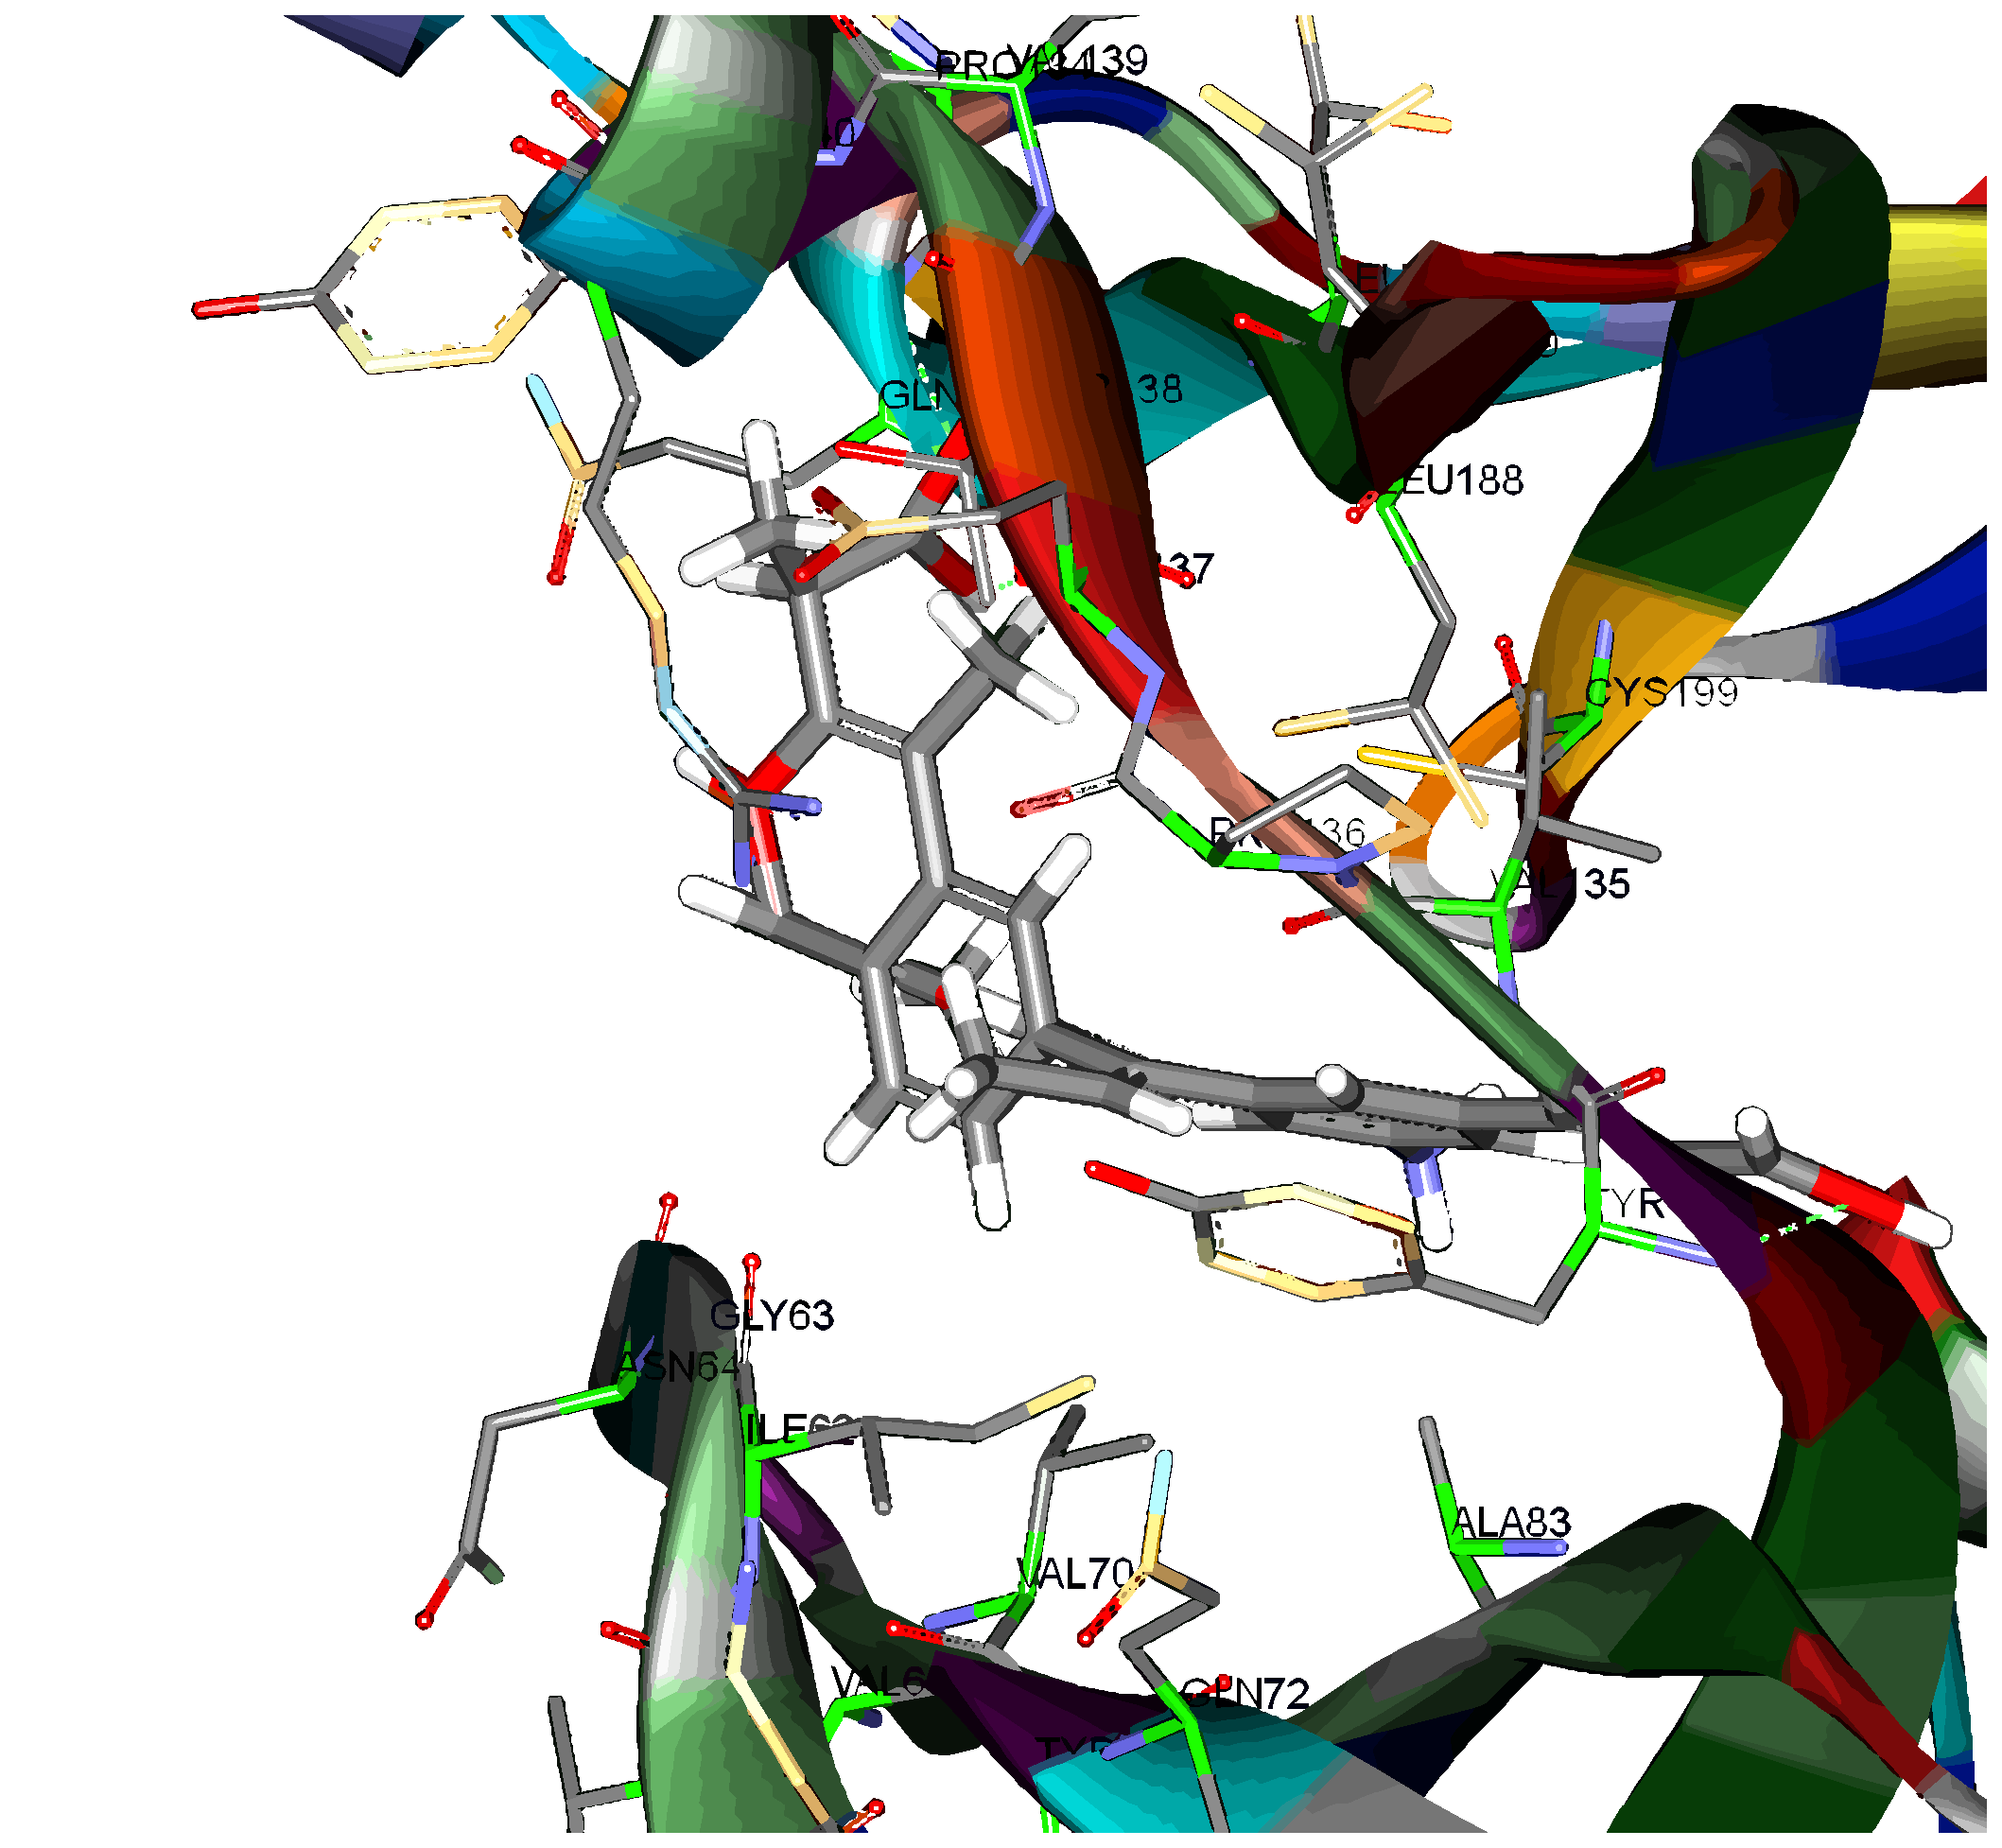
\includegraphics[width=0.31\linewidth]{Figures/Results/1J1B-ZINC01019824-igrow.eps}
}
\caption{The initial ligand and the best ligands generated by AutoGrow and igrow, in the test case of ZINC01019824 docking to GSK3$\beta$. Hydrogen bonds are represented as dotted green lines.}
\label{fig:BestLigands}
\end{figure*}

\begin{figure*}[t]
\centering
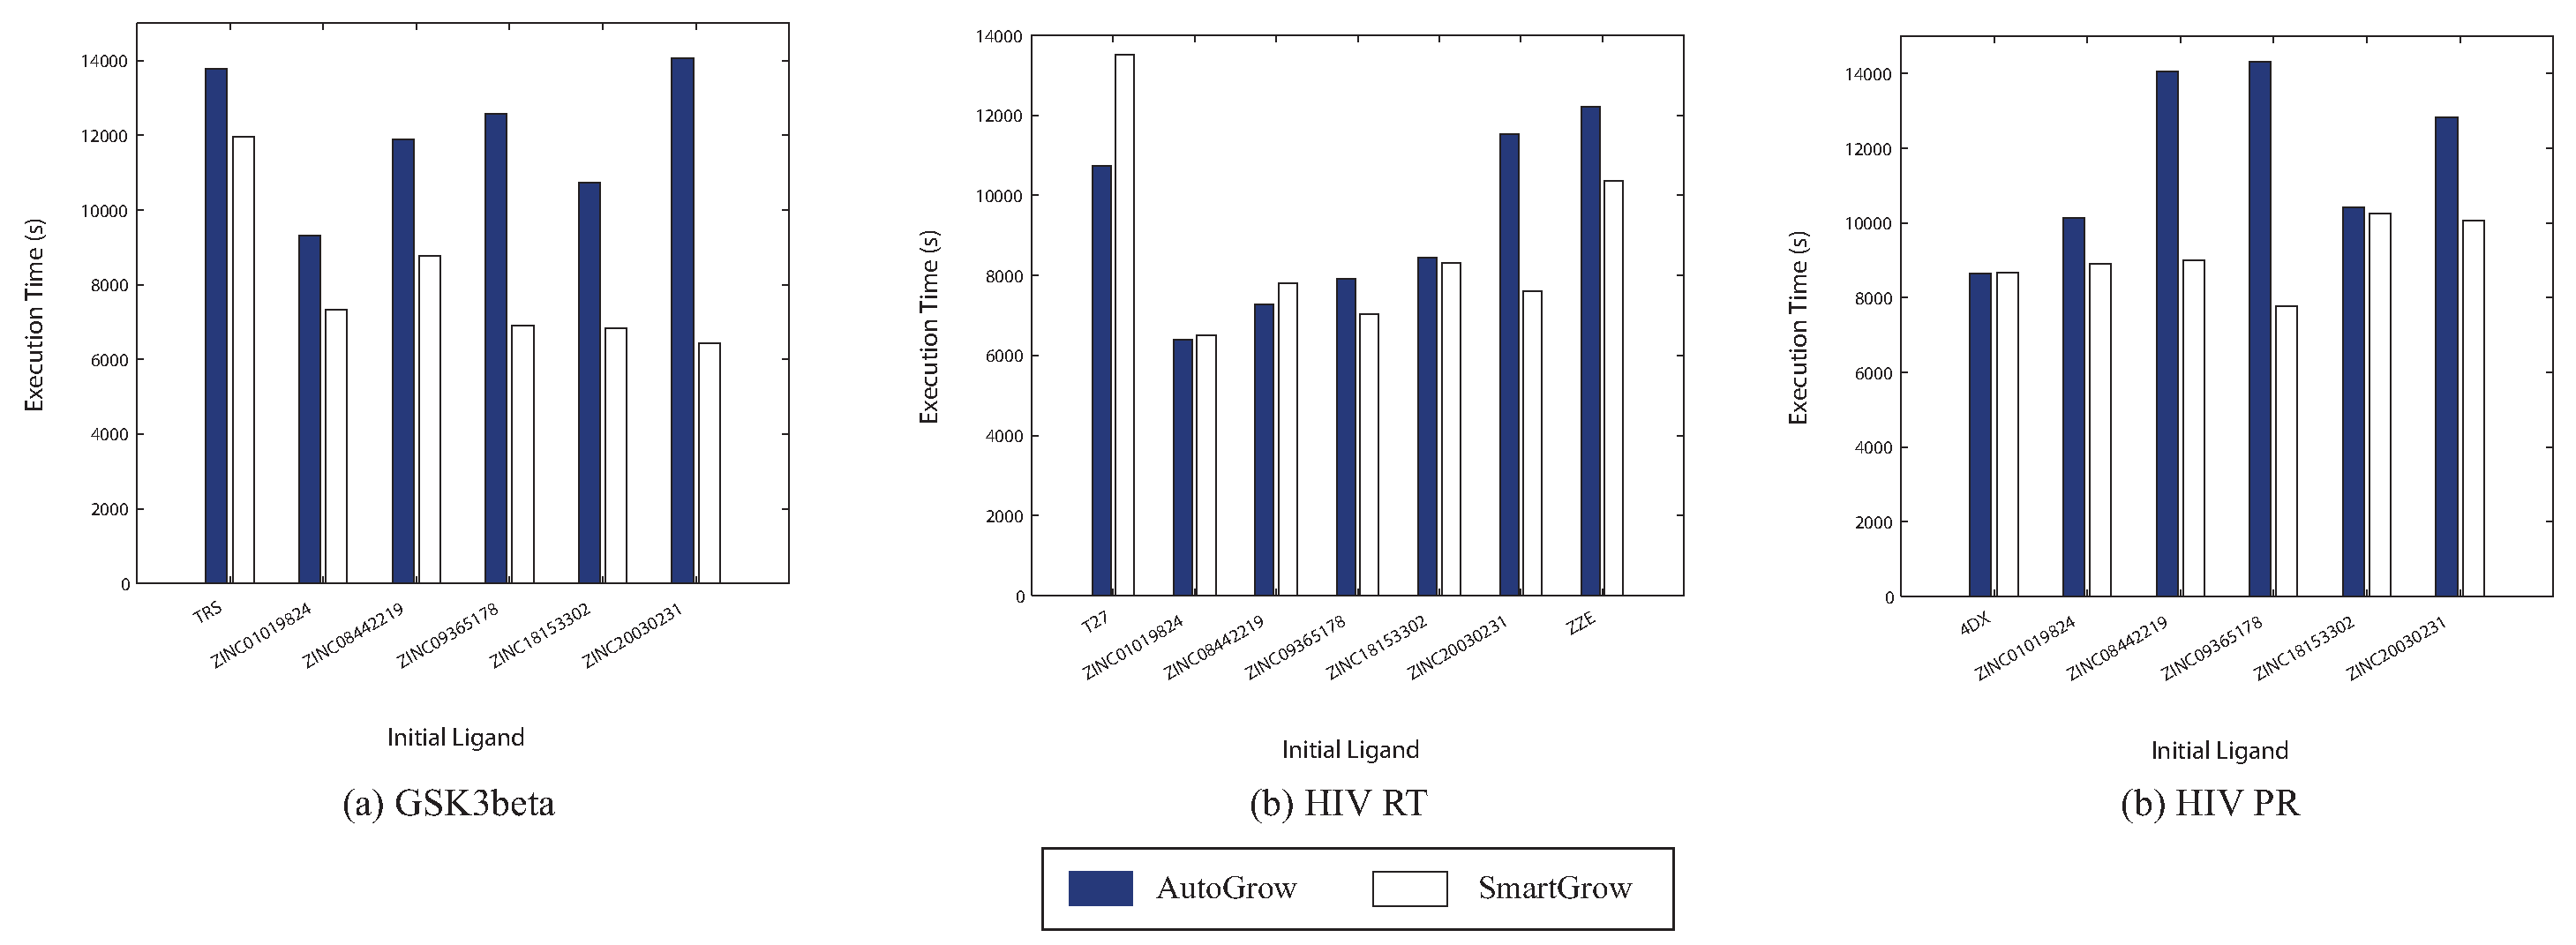
\includegraphics[width=1\linewidth]{Figures/Results/Exeution_time_with_legend.eps}
\caption{Average execution times of AutoGrow and igrow, categorized by 3 receptors.}
\label{fig:ExecutionTime}
\end{figure*}

Figure \ref{subfig:1J1B-ZINC01019824} shows that the initial ligand ZINC01019824 does not form any hydrogen bond with GSK3$\beta$. It contains carbon and hydrogens atoms only, which are neither hydrogen bond donor nor acceptor. Its predicted free energy is -6.9 kcal/mol and its molecular weight is 194 Da.

Figure \ref{subfig:1J1B-ZINC01019824-AutoGrow} shows that the best ligand generated by AutoGrow is predicted to form 4 hydrogens bonds, interacting with Tyr134, Pro136, Gln185, and Asn186 of GSK3$\beta$. Its predicted free energy is -11.9 kcal/mol and its molecular weight is 572 Da, 72\% lower in free energy and 195\% larger in molecular weight than the initial ligand.

Figure \ref{subfig:1J1B-ZINC01019824-igrow} shows that the best ligand generated by igrow is predicted to form 9 hydrogens bonds, interacting with Asp133, Tyr134, Pro184, Gln185 and Asn186 of GSK3$\beta$. Its predicted free energy is -11.2 kcal/mol and its molecular weight is 505 Da, 62\% lower in free energy and 160\% larger in molecular weight than the initial ligand.

\subsection{Free Energy and Molecular Weight}

The goal of fragment-based growing strategy is not to generate one single best ligand, but a population of drug-like ligands to be shortlisted for further verifications by wet lab experiments. Therefore it is more meaningful to dig into the average performance of the best several ligands. Hence the predicted free energies and molecular weights of the best 5 ligands were plotted against generation number in figure \ref{fig:Best5}.

\subsection{Execution Time}

We also measured the execution times of AutoGrow and igrow. Since all the test cases were run for 9 times, their average execution times are shown in figure \ref{fig:ExecutionTime}.

\subsection{Handling Phosphorus}

igrow has built-in support for phosphorus. To examine such capability, from PDB we picked TFO, a phosphorus-containing initial ligand, as an additional test case. The input ligand file contained no PDB CONECT records. The result is shown in the supplementary materials, showing both the best generated ligand and the curves of predicted free energy and molecular weight. In contrast, AutoGrow failed to grow TFO.

\section{Discussions}

Through visualizing the generated ligands in complex of their respective receptors, we found that they are chemically valid, and we are thus of full confidence about the correctness of igrow. An example test case is demonstrated in figure \ref {fig:BestLigands}.
The best ligands generated by igrow have significantly lower molecular weights than those generated by AutoGrow, hence they are more likely to optimize into drugs.

Regarding the average free energies and molecular weights of the best 5 ligands generated by both programs, as shown in figure \ref{fig:Best5}, for most of the cases igrow displays a comparable free energy curve, while its molecular weight curve is remarkably lower than AutoGrow, and seldom exceeds 500, thanks to the guidance of Lipinski's rule of five and the `split' operator.

Regarding the execution time, as shown in figure \ref{fig:ExecutionTime}, igrow outperforms AutoGrow for 14 out of 18 test cases.
For the test case with GSK3$\beta$ as the receptor and ZINC20030231 as the initial ligand, igrow runs as much as 119\% faster than AutoGrow.
For the test case with HIV RT as the receptor and T27 as the initial ligand, although igrow requires 27\% more time, the generated ligands have lower free energies, as shown in figure \ref{fig:Best5}(g).
Averaging all the 18 test cases, in general igrow executes about 30\% faster than AutoGrow.

\section{Availability}

igrow is free and open source under Apache License 2.0. It is written in C++ and available at http://GitHub.com/HongjianLi/igrow.

\section{Conclusions}

We have developed igrow, an efficient tool for computational synthesis of potent ligands.
igrow has inherited the existing mutation and crossover operators from AutoGrow and we have invented two new genetic operators, namely split and merging.
The split operator ensures that ligands will not exceed upper bound.
The merging operator is basically a reversed operator of split which accelerates ligand growing.
igrow implements Lipinski's rule of five to ensure druggability.
The comprehensive results show that igrow outperforms AutoGrow in terms of free energy, molecular weight and execution time.

\bibliographystyle{unsrtnat}
\bibliography{../refworks}

\end{document}
